\chapter{Artes visuais, dança, música e teatro}
\markboth{Módulo 1}{}

\coment{Sugerimos que a primeira leitura do texto seja realizada pelos alunos
individualmente. Depois, faça uma roda de conversa e oriente a discussão
coletiva sobre o texto, fazendo perguntas, como estas:
Como o texto comparou nossa língua e a arte? Essa comparação auxiliou na
compreensão sobre a importância das linguagens artísticas no seu dia a
dia? O que você entendeu por artes plásticas? Quais são as manifestações
das artes plásticas citadas no texto? Quais outras manifestações das
artes plásticas você conhece que não foram citadas no texto? Na
dança, quais manifestações foram citadas pelo texto? Você conhece
outras manifestações de dança? Na música, quais manifestações foram
citadas? Você conhece outras manifestações de música? Quais são os
elementos básicos do teatro?\\
\textbf{Habilidades da BNCC}: EF15AR01, EF15AR02, EF15AR08, EF15AR13,
EF15AR14, EF15AR18}

\colorsec{Habilidades do SAEB}

\begin{itemize}
\item Reconhecer elementos constitutivos das artes visuais, dança, música e
teatro.

\item Identificar formas distintas de artes visuais em diferentes suportes e
mídias.

\item Identificar características do sistema de circulação das artes
visuais, dança, música e teatro em diferentes contextos (teatros,
palcos, museus, galerias, artistas, artesãos, curadores, produtores
etc.).

\item Identificar distintas formas e/ou gêneros de expressão da dança, da
música e do teatro em diferentes contextos e práticas.
\end{itemize}

\conteudo{Na língua portuguesa existem as linguagens verbais e
não verbais. Na linguagem verbal, a comunicação ocorre por meio da palavra (oral ou
escrita). Na linguagem não verbal, a comunicação acontece, por exemplo, por meio de
expressões faciais, mímicas, desenhos, coreografias ou semáforos.

A linguagem é uma atividade humana e pode se manifestar de diversos
modos, dependendo da intenção no momento da
comunicação. Para que você possa se comunicar bem, precisa ter
experiências com variadas formas de comunicação.

Na arte, assim como na língua, a linguagem artística, também
compreendida como atividade humana, manifesta-se de diferentes modos,
por meio de materialidades verbais e não verbais, sempre relacionadas à
história, à cultura e à sociedade de cada grupo. Para que suas
experiências com a arte e suas linguagens sejam enriquecidas, é preciso
ampliar suas práticas artísticas de apreciação, análise, reflexão e
criação.


\begin{itemize}
\item
  \textbf{Artes visuais}
\end{itemize}

São exemplos de artes visuais, ou seja, manifestações artísticas que têm
a expressão relacionada ao sentido da visão: arquitetura, artesanato,
cinema, desenho, escultura, fotografia e pintura.

\begin{itemize}
\item
  \textbf{Dança}
\end{itemize}

São exemplos de danças, manifestações artísticas que têm o corpo como
instrumento de expressão: balé, dança do ventre, forró, frevo, maracatu,
samba e quadrilha.

\begin{itemize}
\item
  \textbf{Música}
\end{itemize}

São exemplos de músicas, manifestações artísticas que têm o som como
meio de expressão: axé, eletrônica, forró, funk, gospel, hip-hop e
samba.

\begin{itemize}
\item
  \textbf{Teatro}
\end{itemize}

Já no teatro, o fazer teatral se dá principalmente pela
reunião de três elementos básicos: o(s) ator(es), o texto e o público.}


\colorsec{Atividades}

\num{1} Você pode utilizar várias partes do seu corpo para produzir sons.
Bata palmas tendo como base as ilustrações de cada tipo de palma e
prestando atenção nos sons que elas produzem: graves ou agudos.

%\begin{longtable}[]{@{}llll@{}}
%\toprule
%Palma concha & Palma estrela & Palma estalada & Palma
%pingo\tabularnewline
%\bottomrule
%\end{longtable}

Agora, numere as palmas da mais grave para a mais aguda. A número 1
corresponderá à palma que produz o som mais grave, e a número 4 corresponderá à que
produz o som mais agudo.

\begin{boxlist}
\boxitem{2} Palma estrela.

\boxitem{4} Palma pingo.

\boxitem{3} Palma estalada.

\boxitem{1} Palma concha.
\end{boxlist}

\coment{A palma concha produz o som mais grave. A palma estrela também produz um
som grave, no entanto menos grave que a palma concha. A palma estalada
produz um som agudo. E o som mais agudo, entre esses tipos de palma, é
produzido pela palma pingo.}

\num{2}  Leia o texto.

\begin{quote}
O carimbó é um ritmo amazônico, típico do Pará, que nasceu das mãos
calejadas e dos pés descalços dos agricultores paraenses. Um ritmo, uma
dança, uma identidade. O nome carimbó ou curimbó vem do tupi:
\emph{curi} é pau oco e \emph{m'bó} é furado.

A união das palavras também batizou o tambor grande e o curimbó se toca
com as pernas abraçando o instrumento. O milheiro e as maracás completam
a sonoridade indígena. A dança de passos miúdos, em roda, também vem da
tradição dos índios, mas não seria de todo Brasil se não tivesse
mistura.

No rebolado está a herança do sangue negro, presente ainda no batuque
acelerado e no som do banjo. Do branco europeu vem o saxofone, a flauta
ou o clarinete. O jeito de dançar em rodopios, com a formação de casais,
é bem português.

{[}...{]}

\fonte{Priscila Brandão. G1. Conheça a história do carimbó. Disponível em:
\emph{https://g1.globo.com/economia/agronegocios/noticia/2015/12/conheca-historia-do-carimbo.html}. Acesso em: 17 mar. 2023.}
\end{quote}

Retire informações do texto para completar o esquema.

%\textless{}Editora, o desenho do esquema deve ser refeito pelo pessoal
%de arte.\textgreater{}

\coment{Para que os alunos possam experimentar os movimentos do carimbó e
ampliar o repertório corporal, indicamos a projeção de vídeos. Entre os
muitos vídeos presentes na internet, sugerimos dois: \emph{Carimbó -- Grupo Sarandeiros -- Dançando na EEFFTO}, disponível em: \emph{https://www.youtube.com/watch?v=mqKD4kM8fHk}
(acesso em: 19 mar. 2023); \emph{Dança do Carimbó Passos básicos Oficina de Dança e Apresentação Cultural}, disponível em: \emph{https://www.youtube.com/watch?v=-0QGO8ua2WE}
(acesso em: 19 mar. 2023).}


\noindent{}Para responder às atividades 3 e 4, leia os conceitos sobre volume
bidimensional e tridimensional.

\begin{mdframed}[linewidth=2pt,linecolor=salmao,backgroundcolor=salmao!20]
\textbf{Bidimensional:} o que tem duas dimensões --- comprimento e largura.

\textbf{Tridimensional:} o que apresenta três dimensões --- comprimento, largura e profundidade.
\end{mdframed}

\num{3} Nas formas de expressão das artes a seguir, assinale B para volume bidimensional ou T para volume tridimensional.

%\begin{longtable}[]{@{}ll@{}}
%\toprule
%\begin{minipage}[b]{0.48\columnwidth}\raggedright\strut
%( D )

%\emph{O estrangeiro} (2009), de Os gêmeos. Vale do Anhangabaú, São
%Paulo, SP (posteriormente removido).

%\textless{}\emph{https://commons.wikimedia.org/wiki/File:OsGemeos.jpg}\textgreater{}\strut
%\end{minipage} & \begin{minipage}[b]{0.48\columnwidth}\raggedright\strut
%( T )

%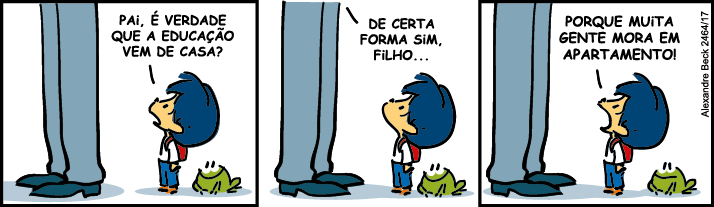
\includegraphics[width=2.92228in,height=1.94792in]{media/image7.png}

%\emph{Cantoneiras} (1975), de Franz Weissmann. Parque Ibirapuera, São
%Paulo, SP.

%\textless{}\href{https://www.flickr.com/photos/arteforadomuseu/5878497076/in/%photolist-9XsQnS-9XsQMC-9XpYcp-vs4Lw7-uxmUkW-9XsSUw-9XsSqs-9XsRU1-9XsRvG-emwHzv}{\emph{%https://www.flickr.com/photos/arteforadomuseu/5878497076/in/%photolist-9XsQnS-9XsQMC-9XpYcp-vs4Lw7-uxmUkW-9XsSUw-9XsSqs-9XsRU1-9XsRvG-emwHzv}}\textgreater{}\strut
%\end{minipage}\tabularnewline
%\midrule
%\endhead
%\begin{minipage}[t]{0.48\columnwidth}\raggedright\strut
%( T )

%\emph{Monumento dos 100 Anos da Imigração Japonesa} (2008), Tomie
%Ohtake, Santos, São Paulo.

%\textless{}\emph{https://commons.wikimedia.org/wiki/File:Monumento_Tomie_Ohtake.jpg}\textgreater{}\strut
%\end{minipage} & \begin{minipage}[t]{0.48\columnwidth}\raggedright\strut
%( D )

%\emph{Um Canto de Meu Ateliê} (1884), de Abigail de Andrade. Coleção
%particular.

%\textless{}https://commons.wikimedia.org/wiki/File:Abigail\_de\_Andrade\_-\_Um\_canto\_no\_meu\_ateli\%C3\%%AA,\_1884.jpg\textgreater{}\strut
%\end{minipage}\tabularnewline
%\bottomrule
%\end{longtable}

\coment{Os Gêmeos, como o próprio nome sugere, são uma dupla de irmãos gêmeos
grafiteiros: Gustavo e Otávio Pandolfo, nascidos em 1974, em São Paulo.
Seus trabalhos fazem parte, principalmente, do cenário paulistano, mas
também estão presentes nos Estados Unidos, na Alemanha,
na Inglaterra e, entre outros países, em Cuba.

Franz Weissman, escultor, desenhista, pintor e professor, nasceu em
Knittelfeld, na Áustria, em 1911. Em 1921, ainda criança, veio morar com
sua família no Brasil. Sua obra tem como base a valorização das formas
geométricas e dos espaços vazados. Foi um dos precursores do movimento
construtivismo no Brasil e criou várias esculturas em espaços públicos.

Abigail de Andrade, pintora e desenhista brasileira, nasceu em 1864, na
cidade de Vassouras (RJ). Ela pintava paisagens, cenas do
cotidiano carioca, retratos, autorretratos e naturezas-mortas. Foi a
primeira mulher a receber uma premiação na Exposição Geral de Belas
Artes, em 1884. No Brasil, naquela época, as mulheres tinham pouco
espaço na aprendizagem artística e eram impedidas de frequentar
oficialmente cursos na Academia Imperial de Belas Artes. Essa
participação só foi possível a partir de 1892.

Tomie Ohtake, pintora, gravurista e escultora, nasceu em Kyoto, no Japão,
em 1913 e chegou ao Brasil em 1936. É uma artista japonesa naturalizada
brasileira e uma das principais representantes do abstracionismo
informal, que busca inspiração no inconsciente e na intuição para
construir arte.}

\num{4}  Dimensão é o espaço que um elemento ocupa. Associe os espaços
  dimensional e tridimensional a suas características.

\begin{multicols}{2}
1. Espaço dimensional.

2. Espaço tridimensional.

\columnbreak

(\rosa{1}) Apresenta figuras dispostas em superfície plana.

(\rosa{1}) Para criar a ilusão de profundidade, utiliza elementos como cores,
linhas, textura.

(\rosa{2}) Os elementos são percebidos por meio de três dimensões: altura,
profundidade e largura.

(\rosa{2}) Possui relevo, o que contribui para a percepção de texturas,
dimensões e espaço.
\end{multicols}


\noindent{}Para responder às atividades 5 e 6, leia o texto.

\begin{quote}
A definição de museu passou por uma significativa mudança. A aprovação
da nova definição de museu se deu durante a 26ª Conferência Geral do
Conselho Internacional de Museus (Icom), em agosto de 2022.


A \textbf{antiga} definição estabelecia:

\emph{O museu é uma instituição permanente sem fins lucrativos, ao
serviço da sociedade e do seu desenvolvimento, aberta ao público, que
adquire, conserva, investiga, comunica e expõe o patrimônio material e
imaterial da humanidade e do seu meio envolvente com fins de educação,
estudo e deleite.}


A \textbf{nova} definição estabelece:

\emph{Um museu é uma instituição permanente, sem fins lucrativos, a
serviço da sociedade, que pesquisa, coleciona, conserva, interpreta e
expõe patrimônio material e imaterial. Abertos ao público, acessíveis e
inclusivos, os museus promovem a diversidade e a sustentabilidade. Atuam
e se comunicam de forma ética, profissional e com a participação das
comunidades, oferecendo experiências variadas de educação,
entretenimento, reflexão e compartilhamento de conhecimento.}

\fonte{Fonte de pesquisa: Museu do Índio. Aprovada nova definição de museu
\emph{https://www.gov.br/museudoindio/pt-br/assuntos/noticias/2022/2022-noticias-durante-o-periodo-de-defeso-eleitoral/aprovada-nova-definicao-de-museu}.
Acesso em: 18 mar. 2023.}
\end{quote}

\num{5}  A experiência do público de museus deve ser segura, democrática e
  diversificada. Transcreva do texto o trecho que contém informações que
  buscam garantir esses direitos.

\linhas{6}
\coment{``Abertos ao público, acessíveis e inclusivos, os museus promovem a
diversidade e a sustentabilidade.''}

\num{6}  Associe as profissões ligadas ao campo dos museus às funções próprias do cargo.

\begin{multicols}{2}

1. Curador.

2. Restaurador.

3. Historiador.

4. Montador.

\columnbreak

(\rosa{4}) Responsável pela montagem da exposição, de acordo com o que foi definido.

(\rosa{3}) Responsável pela pesquisa, pela classificação e pela análise de documentos e objetos do passado.

(\rosa{2}) Responsável pela conservação e pela restauração dos objetos do museu.

(\rosa{1}) Responsável pela concepção e pela supervisão da montagem da exposição.
\end{multicols}


\coment{Explore com os alunos outros profissionais ligados a museus, como: museólogo, educador e orientador de público.}

\num{7}  Observe a imagem e leia o texto.

A fotografia a seguir é um exemplo de arte digital.

%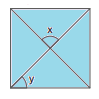
\includegraphics[width=2.97917in,height=2.47913in]{media/image10.png}
%\textless{}\emph{https://commons.wikimedia.org/wiki/File:Carulmare_Have_a_Seat.jpg}\textgreater{}

\emph{Sente-se}, de Carulmare, é uma fotografia que foi tirada em 2009
e editada por meio do \textbf{paint.net}. Paint.net é um aplicativo gratuito para a manipulação e a edição de imagens e fotografias.

Com base na imagem e no texto, o desafio é você fazer arte por meio de uma
fotografia digital. Para isso, você vai precisar de:

\begin{itemize}
\item
  um aparelho de celular e algum aplicativo para tratamento da
  fotografia;
\item
  uma impressora para fazer uma cópia em papel da fotografia;
\item
  determinar, junto com a turma, o tema da exposição;
\item
  definir, junto com a turma, como montar a exposição das fotografias
  digitais para a comunidade escolar.
\end{itemize}

%\begin{longtable}[]{@{}lll@{}}
%\toprule
%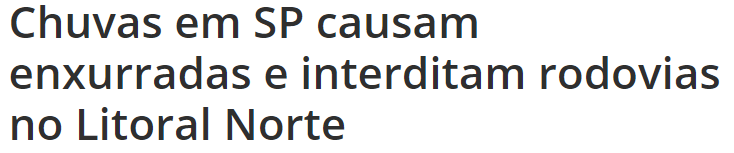
\includegraphics[width=2.05208in,height=1.13481in]{media/image11.png} &
%&\tabularnewline
%\midrule
%\endhead
%Varal de fotos & Mural de fotos & Mosaico de fotos\tabularnewline
%\bottomrule
%\end{longtable}
%
%\textless{}Editora, ilustrar em p\&b. As imagens acima são apenas uma
%referência.\textgreater{}

\coment{A escolha de um tema para a exposição amplia os olhares na fruição dessa
manifestação e a capacidade de simbolizar. São exemplos de temas que
podem fazer parte de uma exposição com foco no olhar do fotógrafo: ``Da
janela da minha casa''; ``Eu de cima ou eu de baixo''; ``Minha comunidade''.
Existem muitos aplicativos para tratamento de fotografias disponíveis na
internet e, possivelmente, os alunos já tiveram acesso a algum
deles. Verifique com eles se já conhecem algum aplicativo, peça a ele que digam qual
indicariam e que justifiquem a indicação. Sugerimos que escolham juntos
apenas um aplicativo, para que as possibilidades de intervenção
artística sobre a foto sejam as mesmas para todos. Alguns aplicativos disponíveis são: Snapseed, Lightroom e VSCO.}


\num{8} Quatro indígenas Guarani Kaiowá fundaram o primeiro grupo
de rap indígena do Brasil: o Brô MC's. De início, eles enfrentaram
a estranheza do público com a ideia de o ritmo ser apropriado pela
etnia, além de enfrentarem, dentro do próprio povoado, os caciques
questionando a empreitada. Agora, ouça -- pelo menos duas vezes --
a música \textit{Terra vermelha}, do Brô MC's, disponível em: \emph{https://www.youtube.com/watch?v=ZwuM0z1IJWo} (acesso em: 19 mar. 2023).
Agora, interprete a letra da canção e, no espaço a seguir, escreva o
que para você é a temática da música.

\linhas{8}
\coment{A música fala de questões indígenas importantes: a demarcação e a perda de terras.}


\num{9} Leia a sinopse do espetáculo teatral infantil \emph{Pinocchio, o musical}.

\begin{quote}
Com roteiro adaptado de um dos maiores clássicos de todos os tempos, o
espetáculo teatral infantil \textit{Pinocchio, o musical} traz uma releitura
contemporânea, que despertará interesse das crianças pela abordagem de
temas relacionados a educação, respeito, obediência aos pais, tudo de
uma forma lúdica, bem humorada e emocionante.

``Como inovação no mercado de peças infantis, trouxemos toda a
ambientação em projeções com realidade virtual, desenvolvidas por um dos
profissionais mais renomados do mercado'', salienta o diretor Luiz
Marcelo Legey.

``Após uma extensa pesquisa, estamos produzindo um musical com roteiro
adaptado de um dos mais tradicionais contos infantis, trazendo cenas e
diálogos contemporâneos, além de reunir uma equipe comprometida com o
objetivo da peça, trazendo muita diversão e uma experiência audiovisual
incrível'', reforçam as diretoras e roteiristas Ana Ferguson e Solange
Bighetti.

{[}...{]}

\fonte{Pinnochio, o musical. Rio no teatro. Disponível em: \emph{https://www.rionoteatro.com.br/pinocchioomusical}.
Acesso em: 19 mar. 2023.}
\end{quote}

Associe o termo ou a expressão do texto com seu significado.

\begin{longtable}[]{@{}lll@{}}
\toprule
Releitura & & Conteúdo de imagens e sons produzidos por
computador.\tabularnewline
\midrule
\endhead
& &\tabularnewline
Realidade virtual & & Texto baseado num material publicado
anteriormente.\tabularnewline
& &\tabularnewline
Roteiro adaptado & & Texto com linguagem do tempo atual.\tabularnewline
& &\tabularnewline
Diálogos contemporâneos & & Nova interpretação, com novo estilo e novas
técnicas, mas sem fugir do tema da obra original.\tabularnewline
\bottomrule
\end{longtable}

\coment{Releitura/nova interpretação, com novo estilo e novas
técnicas, mas sem fugir do tema da obra original. Realidade virtual/
Conteúdo de imagens e sons produzidos por computador. Roteiro adaptado/
Texto baseado num material publicado anteriormente. Diálogos
contemporâneos/ Texto com linguagem do tempo atual.}

\num{10} Utilizando quadrados, círculos e triângulos, crie, em uma folha à parte,
uma obra que represente um objeto, uma pessoa ou um animal. Vale utilizar uma fotografia como referência.

\coment{Resposta pessoal.}

\colorsec{Treino}

\num{1} Observe a imagem e leia a legenda.

%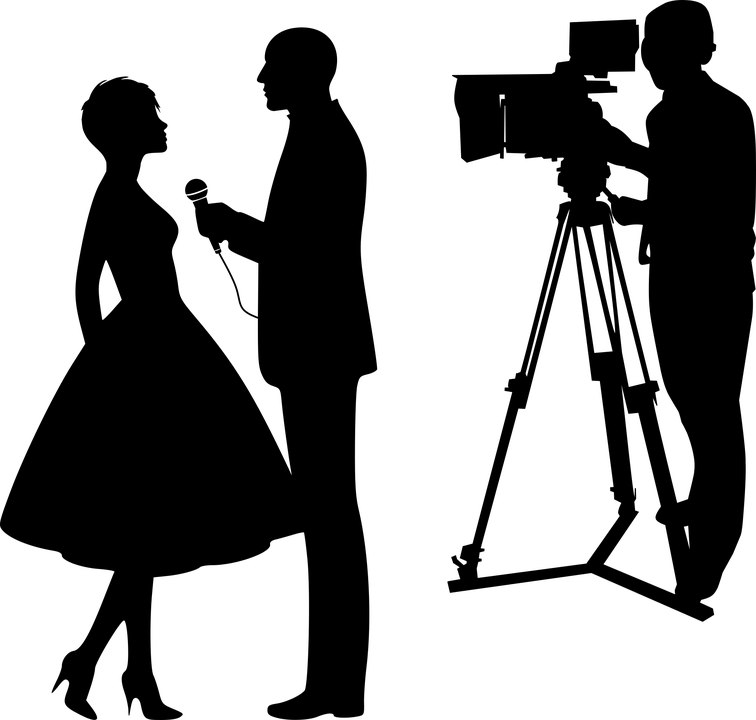
\includegraphics[width=5.90278in,height=3.30625in]{media/image16.png}
%\emph{Invenção da Cor}, \emph{Penetrável Magic Square \#5, De Luxe} (1977), de Hélio Oiticica. Pintura sobre paredes de alvenaria, cobertura de metal e vidro, alambrado, seixo rolado, 15m x 15m x 4,5m.Instituto Cultural Inhotim, Brumadinho, Minas Gerais.
%\emph{https://commons.wikimedia.org/wiki/File:Inhotim_Oiticica_04.jpg}

Assinale a alternativa que corresponde a uma característica da obra.

\begin{escolha}
\item
  Obra colecionável.
\item
  Espaço bidimensional.
\item
  Espaço tridimensional.
\item
  Trabalho em pequeno formato.
\end{escolha}

\coment{SAEB: Reconhecer elementos constitutivos das artes visuais, dança,
música e teatro. BNCC: EF15AR02 -- Explorar e reconhecer elementos constitutivos das artes
visuais (ponto, linha, forma, cor, espaço, movimento etc.).

a) Incorreta. Em geral, as instalações são obras passageiras, com
duração determinada.
b) Incorreta. No espaço dimensional, a obra possui duas dimensões: altura
e largura.
c) Correta. É uma obra com três dimensões: altura, largura e
profundidade.
d) Incorreta. A legenda informa o tamanho da obra: 15 m x 15 m x 4,5 m, ou
seja, é uma obra de grandes dimensões.}

\num{2} Assinale a alternativa que descreve funções do orientador de público em museus.

\begin{escolha}
\item
  Responsável por dar informações para o público sobre as obras
  expostas, em visitas agendadas ou espontâneas.
\item
  Responsável por conservar e restaurar objetos do museu.
\item
  Responsável por pesquisar, classificar e analisar documentos e objetos
  do passado.
\item
  Responsável por supervisionar as áreas expositivas e informar as
  regras de comportamento no museu.
\end{escolha}

\coment{SAEB: Identificar características do sistema de circulação das artes
visuais, dança, música e teatro em diferentes contextos (teatros,
palcos, museus, galerias, artistas, artesãos, curadores, produtores
etc.). BNCC: EF15AR01 -- Identificar e apreciar formas distintas das artes
visuais tradicionais e contemporâneas, cultivando a percepção, o
imaginário, a capacidade de simbolizar e o repertório imagético.

a)  Incorreta. O educador é o responsável por dar informações sobre o que
  está exposto no museu.
b) Incorreta. O restaurador é o profissional responsável pela conservação
  e pela restauração dos objetos.
c) Incorreta. O historiador é o responsável pela pesquisa, pela classificação
  e pela análise de documentos e objetos do passado.
d) Correta. O orientador de público é o responsável por supervisionar as
  áreas expositivas, garantido que as regras de comportamento do museu
  sejam seguidas.}

\num{3}  Leia o texto.

Gênero musical e dança realizada com as canções desse ritmo, pode ser considerado um dos
grandes símbolos da cultura brasileira. E é um patrimônio imaterial do Brasil, além de
ser muito popular no exterior. Surgido no Rio de Janeiro, no começo do século XX, é
resultado da influência da cultura africana no Brasil. O surgimento desse ritmo se deu
nos encontros de afro-brasileiros reunidos para celebrar sua cultura.

Assinale a alternativa que corresponde ao gênero musical descrito no texto.

\begin{escolha}
\item
  Hip-hop.
\item
  Rock.
\item
  Samba.
\item
  Sertanejo.
\end{escolha}

\coment{SAEB: Identificar distintas formas e/ou gêneros de expressão da dança,
da música e do teatro em diferentes contextos e práticas. BNCC: EF15AR13 -- Identificar e apreciar criticamente diversas formas e
gêneros de expressão musical, reconhecendo e analisando os usos e as
funções da música em diversos contextos de circulação, em especial,
aqueles da vida cotidiana.

a)  Incorreta. O hip-hop surgiu nas comunidades afro-americanas na década
  de 1970. Além da música, esse movimento encontra-se representado na
  dança e no grafite.
b) Incorreta. O rock teve sua origem nos Estados Unidos, no final da
  década de 1940.
c) Correta. O samba surgiu nas comunidades afro-brasileiras, no começo do
  século XX. Além de gênero musical, também encontra-se representado na
  dança.
d) Incorreta. O sertanejo é um gênero musical brasileiro, com sua origem
  no início do século XX. Como o próprio nome indica, esse gênero surgiu
  no sertão do Brasil.}

\chapter{O corpo na arte, a arte no corpo, a arte do corpo}
\markboth{Módulo 2}{}

\conteudo{
\textbf{Puxando o fio da conversa...}

Você já parou para pensar na importância do corpo para a arte?

%\textless{}Editora, refazer os balões de pensamento ou utilizar de banco
%de imagens próprio.\textgreater{}

Brincando com essas expressões, podemos analisar quais significados elas
podem conter para você e qualquer outro ser humano que existem em forma
de corpo.

O \textbf{corpo na arte} pode ser, por exemplo, qualquer manifestação
das artes visuais em que o corpo humano esteja representado. Pode ser
uma pintura, uma escultura, um desenho, uma fotografia, um artesanato,
uma xilogravura.

A \textbf{arte no corpo} poder ser uma tatuagem, uma pintura corporal
indígena, uma máscara, uma fantasia.

%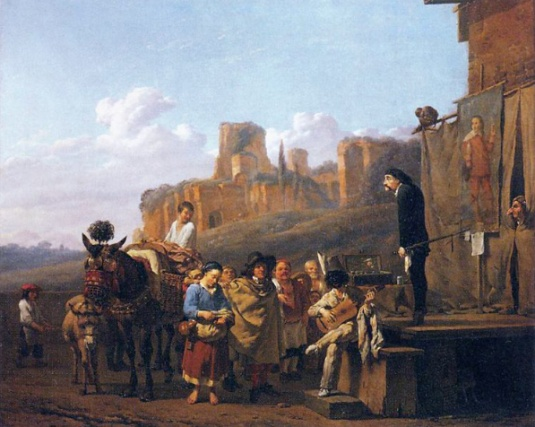
\includegraphics[width=1.27083in,height=1.81148in]{media/image17.jpeg}
%Indígena Kadiwéu (1872), Mato Grosso do Sul, Brasil. Pintura corporal com padrões abstratos.\\ \href{https://commons.wikimedia.org/wiki/File:Kadiweu_woman_1892.jpg}{\emph{https://commons.wikimedia.org/wiki/File:Kadiweu\_woman\_1892.jpg}}

E, \textbf{a arte do corpo}, pode ser encontrada nas pessoas que dançam,
fazem mímica, realizam percussão com o corpo, representam personagens.

E essas são apenas algumas possibilidades.

\textbf{Esticando o fio da conversa...}

Para compreender essas relações do corpo com a arte precisamos entender
que toda manifestação artística faz parte de um momento histórico e
cultural de uma comunidade, região ou país. Quais eram ou são as
crenças, os saberes, as técnicas disponíveis?

E, para finalizar nossa conversa, vai aí uma dica: Para você ampliar
seus conhecimentos sobre a arte é necessário ter experiências artísticas
sensíveis, investigando e refletindo sobre a diversidade presente nas
manifestações, seja como apreciador/interlocutor ou como criador.}

\coment{Sugerimos que a primeira leitura do texto seja realizada pelos alunos em
grupos de quatro a cinco participantes, para que eles possam discutir as
ideias apresentadas no texto. Peça a eles que registrem numa folha
avulsa suas ideias sobre o que significam as expressões: ``corpo na
arte'', ``arte no corpo'', ``arte do corpo'' e, também, sobre momento
histórico e cultural.

A seguir, faça uma roda de conversa e oriente a discussão coletiva sobre
o texto.\\
\textbf{Habilidade BNCC}: (EF15AR03) Reconhecer e analisar a influência
de distintas matrizes estéticas e culturais das artes visuais nas
manifestações artísticas das culturas locais, regionais e nacionais.}

\colorsec{Habilidades SAEB}

\begin{itemize}
\item Identificar as características de instrumentos musicais variados, bem
como o potencial musical do corpo humano.

\item Reconhecer diferentes formas de notação musical.

\item Reconhecer a influência de distintas matrizes estéticas e culturais
nas manifestações das artes visuais, dança, música e teatro na cultura
brasileira.

\item Analisar expressões do teatro e da dança na vida cotidiana.

\item Analisar relações entre as partes corporais e seu todo na estética da dança.
\end{itemize}

\colorsec{Atividades}

Para responder às atividades de 1 a 3, leia o texto.

\begin{quote}
O corpo humano é uma fonte muito rica de sons e pode ser considerado
nosso primeiro instrumento musical. Sentimos a presença do ritmo na
batida de nosso coração, em nossa respiração ou ao caminharmos.
Reconhecemos inúmeros timbres e melodias na exploração de nossa voz e
também na escuta da voz do outro. {[}...{]}

Ao redor do mundo, observa-se uma rica diversidade de formas de canto,
de palmas, de estalos de dedo, de estalos de língua, de sapateados, de
assobios, além dos sons vocais, fonéticos (sons da fala) e onomatopaicos
(reproduz sons de animais, da natureza, entre outros), que conferem à
língua falada de cada região o seu sotaque particular. Essa música
corporal está presente no dia a dia das comunidades, assim como nas suas
danças e festividades. No Brasil existem inúmeros estilos musicais que
se utilizam de sapateados e de palmas em suas manifestações, como: o
coco, o xaxado, o samba de roda, a catira, a chula e o fandango, cujas
coreografias por si só têm um resultado rítmico. {[}...{]}

\fonte{Disponível em:
\emph{http://www.abemeducacaomusical.com.br/revista\_musica/ed5/artigo3.pdf.}
Acesso 20 mar. 2023. (Adaptado para fins didáticos.)}
\end{quote}

\num{1}  Retire do texto os exemplos de manifestações artísticas brasileiras,
  em que as próprias coreografias se utilizam da música corporal?

\reduline{O coco, o xaxado, o samba de roda, a catira, a chula e o fandango.\hfill}

\coment{Depois da primeira leitura do texto e antes da realização da atividade,
explore com os alunos os sons que eles conseguem imitar, tais como: sons
de animais, de instrumentos musicais, da natureza, do ambiente familiar,
entre outros.

Após a realização da atividade, divida a turma em 6 grupos. Cada grupo
será responsável por pesquisar uma manifestação artística diferente:
grupo 1 = coco; grupo 2 = xaxado; grupo 3 = samba de roda; grupo 4 =
catira; grupo 5 = chula e grupo 6 = fandando.

Marque com eles um dia para que os grupos apresentem suas descobertas.

Oriente-os sobre as informações que não podem faltar na pesquisa: as
matrizes históricas e culturais (como se faz presente a matriz africana,
indígena ou europeia), os instrumentos musicais que fazem parte dessa
manifestação e como o corpo é utilizado para produzir sons.

Os vídeos, materiais audiovisuais, são importantes nesse tipo de
pesquisa e você pode indicar alguns. Sugestões:

\begin{itemize}
\item Coco: Vídeo \emph{Coco de Roda Sucena Maringá} -- Ritmos e Manifestações afro-brasileiras. Disponível em: \emph{https://www.youtube.com/watch?v=\_u6nufWq1oM}. Acesso em: 20 mar. 2023.

\item Xaxado: Vídeo \emph{Tropeiros da Borborema} -- Xaxado (Compleo). Disponível
em: \emph{https://www.youtube.com/watch?v=LjlBcX7eyuQ}. Acesso em: 20 mar. 2023.

\item Samba de roda: Vídeo Grupo Sucena -- Samba De Roda -- Ritmos e Manifestações Afro-Brasileiras. Disponível em: \emph{https://www.youtube.com/watch?v=XDDN72SkeRs}. Acesso em: 20 mar. 2023.

\item Catira: Vídeo \emph{Araguaia presente de Deus} -- Catireiros do Araguaia. Disponível
em: \emph{https://www.youtube.com/watch?v=S09RejvYeUQ}. Acesso em: 20 mar. 2023.

\item Chula: Vídeo \emph{Alma Gaúcha} -- Maria Bailarina -- A Chula. Disponível em: \emph{https://www.youtube.com/watch?v=xt\_5\_tfEk3o}. Acesso em: 20 mar. 2023.

\item Fandango: Vídeo \emph{Extras Documentário Fandango} -- dança tradicional
do Paraná (Chico com Grupo Mestre Brasílio). Disponível em: \emph{https://www.youtube.com/watch?v=3eg-vDlkxXc}. Acesso em: 20 mar. 2023.
\end{itemize}

Quando a pesquisa estiver concluída, cada grupo poderá organizar em uma
folha avulsa as informações e, depois, tirar cópias dessas informações
para os colegas dos outros grupos. Assim, ao final, a turma terá dados
de todas as manifestações pesquisadas.

Saeb: -- Reconhecer a influência de distintas matrizes estéticas e
culturais nas manifestações das artes visuais, dança, música e teatro na
cultura brasileira.

BNCC: (EF15AR03) Reconhecer e analisar a influência de distintas
matrizes estéticas e culturais das artes visuais nas manifestações
artísticas das culturas locais, regionais e nacionais.}

\num{2}  Segundo o texto, ``o corpo humano é uma fonte muito rica de sons e
  pode ser considerado nosso primeiro instrumento musical''. Então,
  prepare-se! Você vai seguir as instruções presentes nas ilustrações e
  produzir sons com o corpo.

%\textless{}Editora, as ilustrações a seguir são referências para o ilustrador.\textgreater{}

\begin{longtable}[]{@{}lll@{}}
\toprule
\textbf{1} & \textbf{2} & \textbf{3}\tabularnewline
\midrule
\endhead
Palma costas de mão & Estalo de dedos & Palma estrela\tabularnewline
& &\tabularnewline
\textbf{4} & \textbf{5} & \textbf{6}\tabularnewline
Mãos batendo no peito & Mãos batendo na barriga & Mãos batendo na
coxa\tabularnewline
& &\tabularnewline
\textbf{7} & \textbf{8} & \textbf{9}\tabularnewline
Estalo do lábio & Beijo & Estalo da língua\tabularnewline
\bottomrule
\end{longtable}

\coment{Importante: faça com que seus alunos, em roda, treinem um som de cada
vez, para que possam perceber se o som é agudo ou grave, forte ou fraco,
pode ser executado de forma rápida ou lenta, etc.

A seguir, peça que os alunos executem a sequência de sons e movimentos
do corpo duas vezes, ou seja, duas palmas costas de mão, dois estalos de
dedos, duas palmas estrela, e assim por diante. A seguir, peça que
realizem sequência de três e depois de quatro. Essas sequências podem
começar com movimentos lentos e depois cada vez mais rápidos.

Para mais informações sobre como produzir sons corporais, acessar o
canal YouTube do Barbatuques: \emph{http://www.youtube.com/barbatuques}.
Nele você vai encontrar mais de 290 vídeos para explorar com seus
alunos.

Saeb: -- Identificar as características de instrumentos musicais
variados, bem como o potencial musical do corpo humano.}

\num{3}  A partitura a seguir é para ser interpretada por você junto com seus
  colegas de turma. Para isso, será necessário memorizar o significado
  de cada símbolo.

\coment{Relembre seus alunos que na partitura, assim como nos textos escritos,
lemos em linhas horizontais, da esquerda para a direita e de cima para
baixo.

Saeb: -- Reconhecer diferentes formas de notação musical.}

Para responder às atividades 4 e 5, leia o texto.

\begin{quote}
A dança é uma manifestação social, estética, cultural e simbólica. É uma
forma de comunicação não verbal, onde o corpo é o instrumento básico
para análise, ele é a matriz (a origem) da dança, das performances, dos
gestos plenos de significação consciente e dos movimentos espontâneos.

O balé clássico é uma forma de dança conhecida por prezar pela tradição
e pelo rigor estético. Historicamente, ele nasceu com a Renascença, no século XVI, na
Corte de Médicis, em Paris, refletindo gestos, movimentos e padrões
típicos da época. Mas foi ao final do século XVII que Pierre Beauchamps
definiu as posições básicas do balé clássico, que descrevem todos os
passos.

A partir de então, a técnica clássica
evoluiu pela busca de leveza e agilidade, na qual o
bailarino procura o total domínio do corpo, de seus músculos e de seus
movimentos, de modo a poder utilizá-lo de forma expressiva {[}...{]}.

\fonte{Disponível em:
\emph{http://balletkazanini.blogspot.com/2011/05/o-ballet-classico-e-sua-relevancia.html}.
Acesso em: 20 mar. 2023. (Adaptado para fins didáticos)}
\end{quote}

\num{4}  Complete o esquema com informações retiradas do texto.

%\textless{}Editora, refazer o esquema.\textgreater{}

\begin{longtable}[]{@{}lllllll@{}}
\toprule
& & \textbf{Dança} & & &\tabularnewline
\midrule
\endhead
& & & & & &\tabularnewline
& & Instrumento & & &\tabularnewline
& & & & & &\tabularnewline
& & Corpo & & &\tabularnewline
& & & & & &\tabularnewline
& & Manifestação & &\tabularnewline
& & & & & &\tabularnewline
Social & & Estética & & Cultural & & Simbólica\tabularnewline
\bottomrule
\end{longtable}

\coment{Saeb: -- Reconhecer a influência de distintas matrizes estéticas e
culturais nas manifestações das artes visuais, dança, música e teatro na
cultura brasileira.

BNCC: (EF15AR03) Reconhecer e analisar a influência de distintas
matrizes estéticas e culturais das artes visuais nas manifestações
artísticas das culturas locais, regionais e nacionais.}

\num{5}  Associe a descrição do passo de balé à sua imagem.

%\begin{longtable}[]{@{}ll@{}}
%\toprule
%\begin{minipage}[b]{0.48\columnwidth}\raggedright\strut
%\begin{enumerate}
%\def\labelenumi{\arabic{enumi}.}
%\item
  %\emph{\textbf{Cambré}} -- Arqueado.
%\end{escolha}
%
%Dobrar o corpo a partir da cintura, para a frente, para trás ou para os
%lados, a cabeça acompanha o movimento.\strut
%\end{minipage} & \begin{minipage}[b]{0.48\columnwidth}\raggedright\strut
%( 2 )
%
%%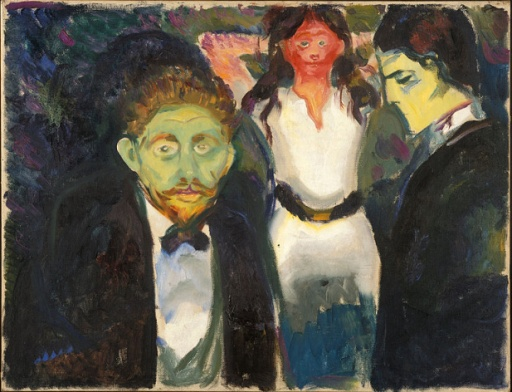
\includegraphics[width=1.42708in,height=2.14181in]{media/image27.jpeg}
%
%\textless{}\emph{http://pixabay.com/pt/photos/balé-homem-dançarino-gracioso-108698/}\textgreater{}\strut
%\end{minipage}\tabularnewline
%\midrule
%\endhead
%\begin{minipage}[t]{0.48\columnwidth}\raggedright\strut
%\begin{enumerate}
%\def\labelenumi{\arabic{enumi}.}
%\item
  %\emph{\textbf{Jeté}} -- Jogado, atirado.
%\end{escolha}
%
%Um pulo de uma perna para qualquer direção.\strut
%\end{minipage} & \begin{minipage}[t]{0.48\columnwidth}\raggedright\strut
%( 3 )
%
% 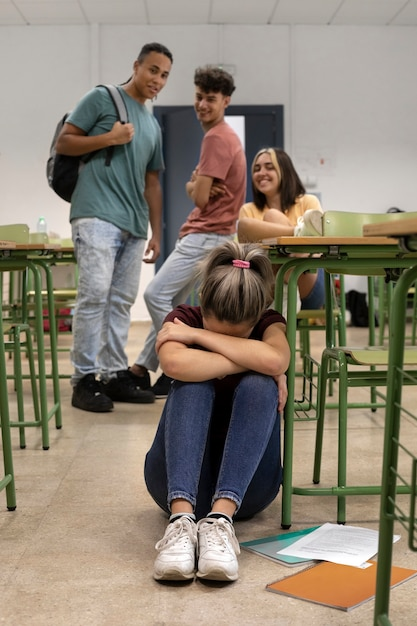
\includegraphics[width=2.13542in,height=2.41816in]{media/image28.jpeg}
%
%\textless{}http://pixabay.com/pt/photos/balé-dança-pessoas-garota-2564266/\textgreater{}\strut
%\end{minipage}\tabularnewline
%\begin{minipage}[t]{0.48\columnwidth}\raggedright\strut
%\begin{enumerate}
%\def\labelenumi{\arabic{enumi}.}
%\item
  %\emph{\textbf{Arabesque}} -- Arabesco.
%\end{escolha}

%É uma das poses básicas do ballet, onde o bailarino fica apoiado numa só
%perna que pode estar na vertical ou em demi plié, com a outra perna
%estendida para trás e em ângulo reto com ela, sendo que os braços estão
%estendidos em várias posições harmoniosas criando a linha mais longa
%possível da ponta dos dedos da mão à dos pés. Os ombros devem ser
%mantidos retos em frente à linha de direção.\strut
%\end{minipage} & \begin{minipage}[t]{0.48\columnwidth}\raggedright\strut
%( 4 )
%
%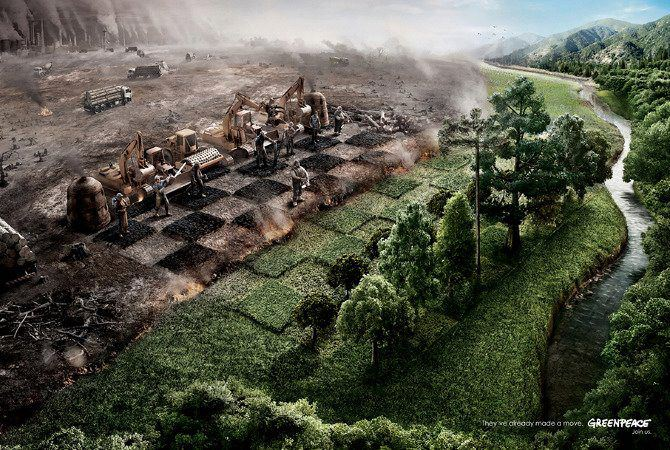
\includegraphics[width=1.66667in,height=2.51572in]{media/image29.jpeg}
%
%\textless{}http://pixabay.com/pt/photos/fêmea-balé-dança-dançarino-437990/\textgreater{}\strut
%\end{minipage}\tabularnewline
%\begin{minipage}[t]{0.48\columnwidth}\raggedright\strut
%\textbf{4. \emph{Derriére}} -- Atrás.
%
%Movimento, passo ou a colocação de um membro atrás do corpo.\strut
%\end{minipage} & \begin{minipage}[t]{0.48\columnwidth}\raggedright\strut
%( 1 )
%
%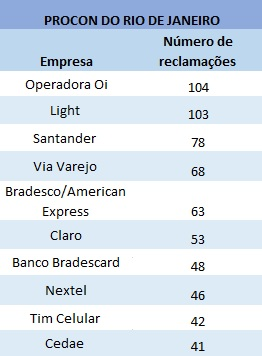
\includegraphics[width=1.81209in,height=1.88542in]{media/image30.jpeg}
%
%\textless{}\emph{http://pixabay.com/pt/photos/danse-classique-balé-dança-5381506/}\textgreater{}\strut
%\end{minipage}\tabularnewline
%\bottomrule
%\end{longtable}
%
%Fonte: \emph{https://escolaartedanca.com.br/dicionario-de-ballet}. Acesso
%em: 20 mar. 2023.

\coment{Informe aos seus alunos que os nomes das técnicas do balé clássico,
nomes dos passos, ações e mímicas, são do idioma francês. Os franceses
foram os primeiros a codificar as técnicas e essa tradição se mantém até
os dias atuais.

Saeb: -- Analisar relações entre as partes corporais e seu todo na
estética da dança.}

Para responder às atividades 6 e 7, leia o texto.

\begin{quote}
A trupe teatral \emph{Esquadrão da} \emph{Vida} foi fundada em 1979, em
Brasília. Com intervenções no formato de teatro de rua, foi pioneira na
abordagem de temas que marcariam a vida cultural brasileira: o resgate e
a valorização da cultura popular; a denúncia da exclusão de parte da
população dos espaços culturais tradicionais; a subversão bem-humorada
do espaço público; e a conscientização ecológica. O \emph{Esquadrão da
Vida} trabalha com um teatro livre de academicismo, incorporando
elementos expressivos das festas populares e de saltimbancos, como
acrobacia, música e dança.

A importância do teatro de rua numa cidade burocrática como Brasília é
gritante, já que altera a atmosfera do espaço público urbano. A morte de
seu fundador, Ary Pára-Raios, suspendeu as atividades da trupe entre
2003 e 2007. Mas, após esse período, o Esquadrão da Vida retornou
fortalecido. Agora, com quase 40 anos de existência, é encabeçado por
Maíra Oliveira, filha de Ary.

\fonte{Disponível em:
\emph{https://brasilia.memoriaeinvencao.com/esquadrao-da-vida}. Acesso
em: 21 mar. 2023.}
\end{quote}

\num{6}  Complete o esquema com informações retiradas do texto.

%\textless{}Editora, refazer a ilustração do esquema.\textgreater{}

\coment{Saeb: -- Analisar expressões do teatro e da dança na vida cotidiana.

BNCC: (EF15AR03) Reconhecer e analisar a influência de distintas
matrizes estéticas e culturais das artes visuais nas manifestações
artísticas das culturas locais, regionais e nacionais.}

\num{7} Observe a imagem e responda: Qual o perfil do público que participa de uma apresentação de teatro em espaços públicos e abertos?

%\begin{longtable}[]{@{}ll@{}}
%\toprule
%\begin{minipage}[t]{0.48\columnwidth}\raggedright\strut
%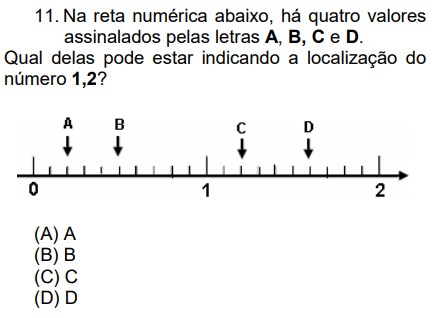
\includegraphics[width=2.42708in,height=1.87061in]{media/image31.png}
%
%O grupo de teatro \emph{Esquadrão da vida} durante apresentação em
%Brasília, DF, Brasil.
%\emph{https://commons.wikimedia.org/wiki/File:Esquadrao_da_vida.jpg}\strut

\reduline{Resposta pessoal. Deve apresentar conteúdo semelhante a este: Todas as
pessoas que passam pela rua, que não foram convidadas, não compraram
ingressos, mas se depararam com a apresentação no seu cotidiano. São
espectadores/participantes ativos, de todas as idades, gêneros,
raça/etnia, classe social.\hfill}

\coment{Saeb: -- Analisar expressões do teatro e da dança na vida cotidiana.}

Para responder às atividades 8 e 9, leia o texto.

%\begin{longtable}[]{@{}ll@{}}
%\toprule
%\begin{minipage}[t]{0.48\columnwidth}\raggedright\strut
%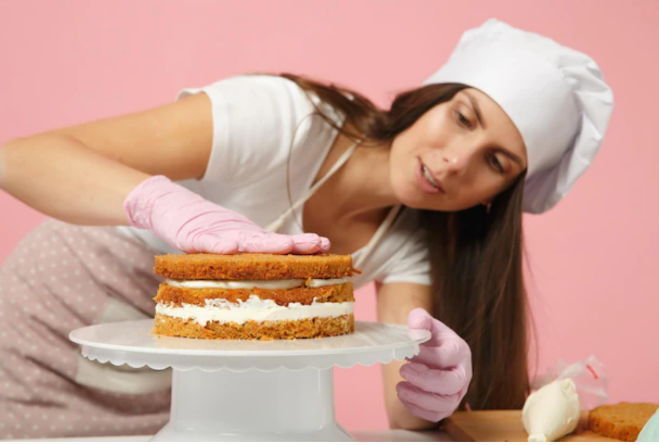
\includegraphics[width=1.93750in,height=2.90020in]{media/image32.png}
%
%Karai Guarani com Maracá
%\emph{https://commons.wikimedia.org/wiki/File:Xam\%C3\%A3_guarani.jpg}

\begin{quote}
O maracá é um dos instrumentos musicais indígenas mais conhecidos, sendo
seu nome muitas vezes utilizado como uma designação genérica para
chocalhos. Consiste numa cabaça seca e oca com pequenas pedras, caroços
ou sementes em seu interior, colocada na extremidade de um bastão,
normalmente feito de madeira.

Em determinados casos, o instrumento é atravessado pela haste e
apresenta dois cabos. Alguns maracás são ornamentados com penas no
suporte e outros têm a cabaça ornada com desenhos. Entre as mais
diversas populações indígenas, o maracá é utilizado geralmente para
marcar o ritmo do canto e da dança durante cerimônias, festividades,
ritos e outras manifestações culturais e sociais. {[}...{]}

\fonte{Disponível em:
\emph{https://www.gov.br/funai/pt-br/assuntos/noticias/2022-02/cultura-saiba-mais-sobre-o-maraca-instrumento-musical-indigena}.
Acesso em: 21 mar. 2023.}
\end{quote}

\num{8}  Complete a tabela com informações retiradas do texto.

\begin{longtable}[]{@{}ll@{}}
\toprule
\textbf{Maracá -- instrumento musical de origem indígena}\tabularnewline
\midrule
\endhead
Material utilizado na confecção & Para que é utilizado\tabularnewline
\begin{minipage}[t]{0.48\columnwidth}\raggedright\strut
\begin{itemize}
\item
  cabaça
\item
  pedras, caroços ou sementes
\item
  madeira
\item
  penas
\end{itemize}\strut
\end{minipage} & \begin{minipage}[t]{0.48\columnwidth}\raggedright\strut
Para marcar o ritmo do canto e da dança durante cerimônias,
festividades, ritos e outras manifestações culturais e sociais.\strut
\end{minipage}\tabularnewline
\bottomrule
\end{longtable}

\coment{Saeb: -- Identificar as características de instrumentos musicais
variados, bem como o potencial musical do corpo humano.}

\num{9}  Assinale a alternativa que corresponde à forma como o som do maracá é produzido.

\begin{boxlist}
\boxitem{\white{X}} Instrumento que soa pela vibração do ar no seu interior.

\boxitem{\white{X}} Instrumento que soa pela vibração de uma membrana esticada em algum suporte.

\boxitem{X} Instrumento que soa pela própria vibração do instrumento.

\boxitem{\white{X}} Instrumento que soa pela vibração de cordas tensionadas.
\end{boxlist}

\coment{Saeb: -- Identificar as características de instrumentos musicais
variados, bem como o potencial musical do corpo humano.}

\num{10} Leia a descrição de um instrumento.

\begin{quote}
Está entre os principais instrumentos musicais brasileiros, uma vez que
é bastante utilizado em alguns estilos de música bem tradicionais do
Brasil, tais como: o pagode e o samba.

Esse instrumento chegou em território nacional por meios dos portugueses
e foi muito usado pelos negros escravizados na capoeira.

\fonte{Disponível em:
\emph{https://www.sabra.org.br/site/instrumentos-musicais-2/}. Acesso em:
21 mar. 2023. (Adaptação para fins didáticos.)}
\end{quote}

Marque a imagem que corresponde à descrição.

( )
Berimbau

%\emph{https://img.freepik.com/fotos-gratis/homem-sem-camisa-praticando-capoeira-na-praia-com-arco-de-madeira_23-2149890199.jpg?w=740\&t=st=1679451646exp=1679452246hmac=9946212703fb0291ca4b153334d370a2e8f666a3d2128e3dad3759f0586e2098}\strut

( X )
Pandeiro
%\emph{https://img.freepik.com/fotos-gratis/homem-sem-camisa-praticando-capoeira-na-praia-com-pandeiro_23-2149890207.jpg?w=740\&t=st=1679452231exp=1679452831hmac=ad748185fdf833d407e42c46bea88414dbe99852cfcae32c868f104ec6a3d177}\strut

( )
Cavaquinho
%\emph{https://commons.wikimedia.org/wiki/File:Cavaquinho2.JPG?uselang=pt}\strut


( )
Violão
%\emph{https://img.freepik.com/fotos-gratis/retrato-de-menina-bonita-violao-jogo-com-bicicleta-em-natureza_1150-12842.jpg?w=740\&t=st=1679453252exp=1679453852hmac=a8b0f84c5df0f44f8ab082adf749f28dbc1a83ff77519004f771ee815905c6dd}

\coment{Saeb: -- Identificar as características de instrumentos musicais
variados, bem como o potencial musical do corpo humano.

Saeb: -- Reconhecer a influência de distintas matrizes estéticas e
culturais nas manifestações das artes visuais, dança, música e teatro na
cultura brasileira.}

\colorsec{Treino}

\num{1} Observe a imagem de cinco posições do balé clássico.

%Editora, escolhi uma imagem que representa o homem no balé. Essa escolha
%foi proposital. Ela servirá de base para o ilustrador. Os textos que
%acompanham a imagem na ordem em que aparecem são:
%
%Título: Posições fundamentais de pernas/pés
%
%Texto 1ª imagem: 1ª posição
%
%Texto 2ª imagem: 1ª posição vista de lado
%
%Texto 3ª imagem: 2ª posição
%
%Texto 4ª imagem: 3ª posição
%
%Texto 5ª imagem: 4ª posição vista de lado
%
%Texto 6ª imagem: 4ª posição
%
%Texto 7ª imagem: 5ª posição

%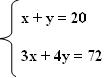
\includegraphics[width=5.90556in,height=2.50359in]{media/image37.jpeg}

Assinale a alternativa que apresenta características técnicas do balé
clássico no Brasil e no mundo.

\begin{escolha}
\item
  Na prática do balé, o excesso de exercícios e repetições podem causar
  lesões nos ossos e músculos.
\item
  No balé são utilizadas dois tipos de sapatilha: a ``de meia ponta'' e
  a ``de ponta''.
\item
  O balé clássico surgiu no século XV e fazia parte do entretenimento
  dos nobres italianos.
\item
  O bale clássico é uma modalidade de dança que, geralmente, segue o
  mesmo padrão de posições no Brasil e em qualquer parte do mundo.
\end{escolha}

\coment{Nível: difícil.

Saeb: -- Analisar relações entre as partes corporais e seu todo na
estética da dança.

Resposta:

a) Incorreta. Essa alternativa refere-se a problemas de saúde vinculados
a prática excessiva ou incorreta das técnicas do balé.
b) Incorreta. As sapatilhas são peças do vestuário clássico dos
dançarinos de balé e auxiliam na execução correta dos movimentos.
c) Incorreta. Fala sobre o contexto histórico e social para a prática do
balé naquela época.
d) Correta. O ensino tradicional do balé clássico valoriza o domínio dos
movimentos e técnicas exaustivamente.}

\num{2} Observe a imagem.

%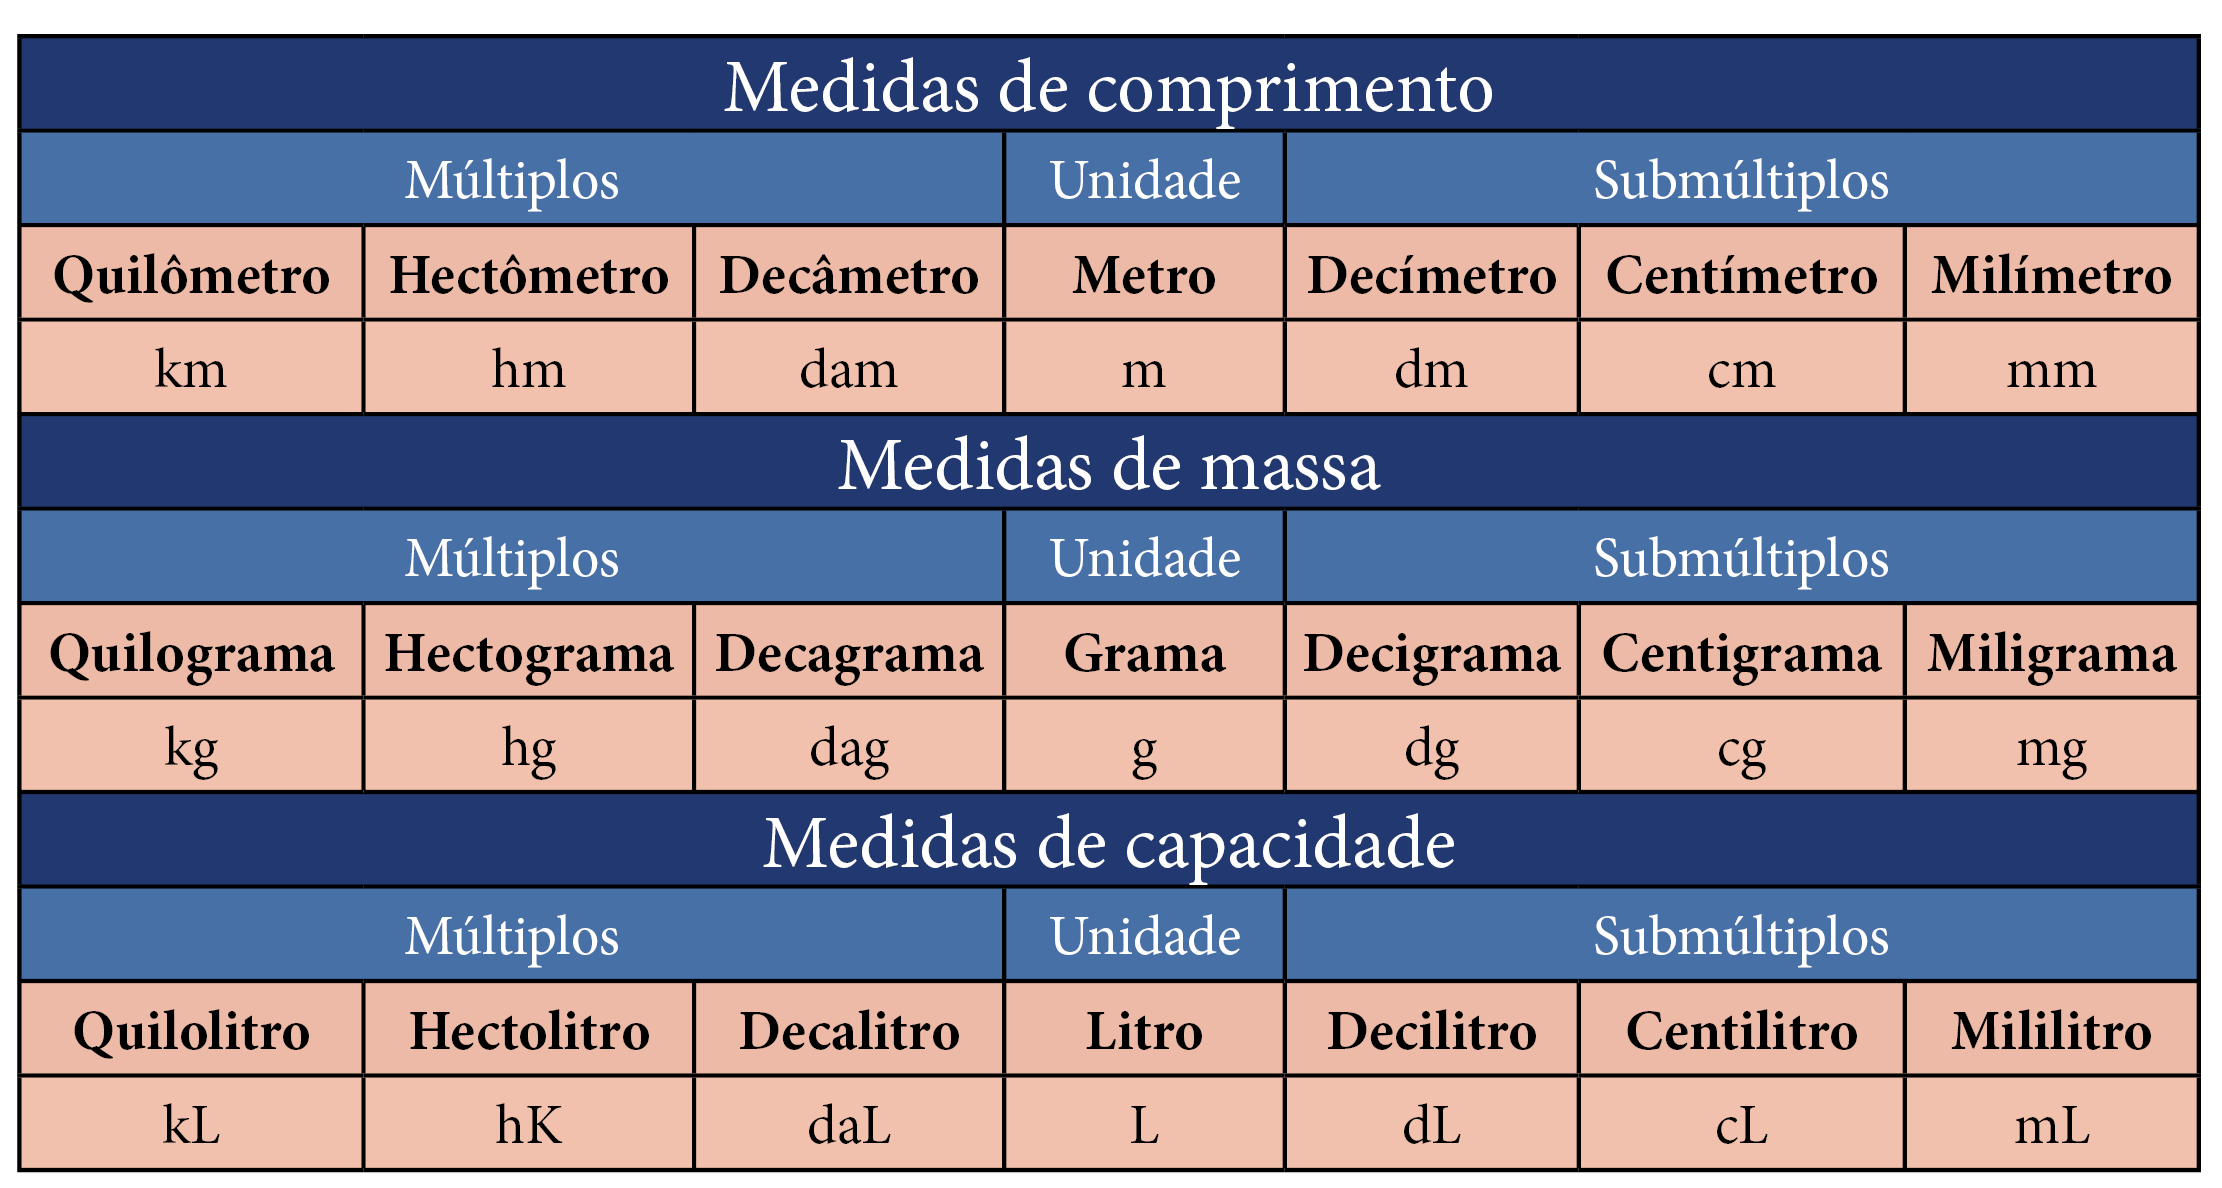
\includegraphics[width=4.13542in,height=2.68401in]{media/image38.png}

Flauta uruá. Aldeia Kamaiurá, Alto\_Xingu.

\emph{https://commons.wikimedia.org/wiki/File:Ift00054vb00.jpg}

Assinale a alternativa que corresponde à forma como o som da flauta uruá é produzido.

\begin{escolha}
\item
  Pela própria vibração do instrumento.
\item
  Pela vibração de cordas tensionadas.
\item
  Pela vibração de uma membrana esticada em algum suporte.
\item
  Pela vibração do ar no seu interior.
\end{escolha}

\coment{Nível: fácil.

Saeb: -- Identificar as características de instrumentos musicais
variados, bem como o potencial musical do corpo humano.

Resposta:

a) Incorreta. São os idiofones que produzem som através da vibração de
seu próprio corpo. Exemplo: Sino.
b) Incorreta. São os cordofones que produzem som através da vibração das
cordas. Exemplo: violino.
c) Incorreta. São os membrafones que produzem som por meio de uma
membrana. Exemplo: tambor.
d) Correta. A flauta é classificada como aerofone, ou seja, produz som
através da vibração do ar.}

\num{3}  Leia o texto.

\begin{quote}
O Samba de Roda do Recôncavo Baiano é um misto de expressão musical,
coreografia característica, poética abrangente, presente em momentos
festivos. É uma das principais manifestações culturais engendrada em
solo brasileiro. {[}...{]}

Seus primeiros registros, com esse nome e com muitas características que
ainda hoje o identificam, datam dos anos 1860. Atualmente, reúne as
tradições culturais transmitidas por africanos escravizados e seus
descendentes, que incluem o culto aos orixás e caboclos, o jogo da
capoeira e a chamada comida de azeite. A herança negro-africana no samba
de roda se mesclou de maneira singular a traços culturais trazidos pelos
portugueses (principalmente viola e pandeiro) e à própria língua
portuguesa nos elementos de suas formas poéticas. {[}...{]}

\fonte{Disponível em:
\emph{http://www.cultura.ba.gov.br/2020/03/17464/Samba-de-Roda-do-Reconcavo-baiano-passa-a-ser-Patrimonio-Imaterial-do-Estado.html}.
Acesso em: 21 mar. 2023.}
\end{quote}

Assinale a alternativa que corresponde à principal matriz estética e
cultural do Samba de Roda do Recôncavo Baiano.

\begin{escolha}
\item
  Africana.
\item
  Asiática.
\item
  Europeia.
\item
  Indígena.
\end{escolha}

\coment{Nível: médio.

Saeb: -- Reconhecer a influência de distintas matrizes estéticas e
culturais nas manifestações das artes visuais, dança, música e teatro na
cultura brasileira.

BNCC: (EF15AR03) Reconhecer e analisar a influência de distintas
matrizes estéticas e culturais das artes visuais nas manifestações
artísticas das culturas locais, regionais e nacionais.

Resposta:

a) Correta. A principal matriz estética e cultural do Samba de Roda do
Recôncavo Baiano é a africana.
b) Incorreta. Fazem parte da cultura asiática países como a China,
Japão, Índia, Coreia do Norte e do Sul, entre outros.
c) Incorreta. Apesar de a cultura europeia fazer parte das matrizes
estéticas e culturais do Samba de Roda do Recôncavo Baiano, a matriz
principal é a africana.
d) Incorreta. O texto não inclui a matriz estética e cultural indígena.}

\chapter{Patrimônio Cultural}
\markboth{Módulo 3}{}

\conteudo{
\textbf{Puxando o fio da conversa...}

Para começar a conversa observe cada imagem a seguir.

%\begin{longtable}[]{@{}lll@{}}
%\toprule
%\begin{minipage}[b]{0.32\columnwidth}\raggedright\strut
%Vestimenta do século XVIII.
%
%\emph{https://commons.wikimedia.org/wiki/File:MA-Lebrun.jpg}\strut
%\end{minipage} & \begin{minipage}[b]{0.32\columnwidth}\raggedright\strut
%Trajes típicos bolivianos.
%
%\emph{https://commons.wikimedia.org/wiki/File:Altiplano_bolivie769m.jpg}\strut
%\end{minipage} & \begin{minipage}[b]{0.32\columnwidth}\raggedright\strut
%Chinesa comendo com palitinhos.
%
%\emph{https://commons.wikimedia.org/wiki/File:Lady_eating_xizo_long_bao_in_Shanghai.jpg?uselang=pt}\strut
%\end{minipage}\tabularnewline
%\midrule
%\endhead
%\begin{minipage}[t]{0.32\columnwidth}\raggedright\strut
%
\includegraphics[width=1.25000in,height=1.87500in]{media/image42.jpeg}
%
%Criança aprendendo a fazer pão de queijo com o pai.
%
%\emph{https://cdn.pixabay.com/photo/2017/01/04/03/27/baking-1951256_960_720.jpg}\strut
%\end{minipage} & \begin{minipage}[t]{0.32\columnwidth}\raggedright\strut
%Grupo mexicano de dança -- Festa dos Mortos.
%
%\emph{https://commons.wikimedia.org/wiki/File:New_generations.JPG?uselang=pt}\strut
%\end{minipage} & \begin{minipage}[t]{0.32\columnwidth}\raggedright\strut
%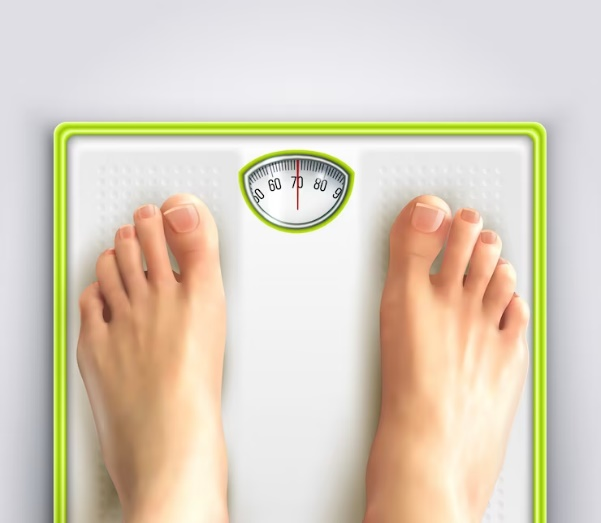
\includegraphics[width=1.97205in,height=1.54167in]{media/image44.jpeg}
%
%Fotos de família.
%
%\emph{https://cdn.pixabay.com/photo/2016/06/28/02/15/retro-1483781_960_720.jpg}\strut
%\end{minipage}\tabularnewline
%\bottomrule
%\end{longtable}

Você viu imagens de épocas diferentes da sua, concorda? Outras você pode
reconhecer como da sua época.

Pôde observar e analisar trajes típicos de outro país, vestimenta do
século XVIII, talheres (palitinhos) típicos da China, conhecer o nome de
uma festa mexicana.

Além disso, você viu objetos, como fotografias, que alguma pessoa
escolheu para guardar e também viu uma criança aprendendo o modo de
fazer pão de queijo.

Cada uma dessas imagens pode fazer parte do patrimônio de uma pessoa, de
um grupo, de um país e revelam detalhes de cada cultura.

\textbf{Esticando o fio da conversa...}

A cultura compreende as visões de mundo, as crenças, os saberes e
fazeres, transmitidos de geração a geração.

O patrimônio é tudo aquilo que escolhemos para guardar: histórias,
objetos, memórias. Podemos unir essas duas ideias e dizer, de forma
simplificada, que o patrimônio cultural compreende os bens materiais
(que se podem tocar) e imateriais (não se podem tocar) que cada grupo,
região ou país escolheu para preservar, conservar, proteger.

São exemplos de bens materiais: fotografias, vestimentas, obras de arte,
cidades, talheres. São exemplos de bens imateriais: culinária, danças,
festas, lendas.}

\coment{
Sugerimos que a primeira leitura do texto seja realizada por você e
acompanhada pelos alunos, numa roda de conversa. Primeiro faça com que
os alunos observem e analisem as imagens e legendas, uma de cada vez,
buscando encontrar diferenças e semelhanças com a cultura brasileira e
contemporânea. Depois, leia um parágrafo de cada vez, discutindo com
eles as ideias e informações apresentadas.

Ao final da conversa, abra espaço para que os alunos esclareçam suas
dúvidas.\\
\textbf{Habilidade BNCC}: (EF15AR25) Conhecer e valorizar o patrimônio
cultural, material e imaterial, de culturas diversas, em especial a
brasileira, incluindo-se suas matrizes indígenas, africanas e europeias,
de diferentes épocas, favorecendo a construção de vocabulário e
repertório relativos às diferentes linguagens artísticas.}

\colorsec{Habilidade SAEB}

\begin{itemize}
\item Avaliar nas linguagens artísticas a diversidade do patrimônio cultural
da humanidade (material e imaterial), em especial o brasileiro, a partir
de suas diferentes matrizes.
\end{itemize}

\colorsec{Atividades}

Para responder às atividades 1 e 2, leia o texto.

\begin{quote}
Os marajoaras vieram do noroeste da América do Sul e chegaram à Ilha de
Marajó, por volta de 400 d.C. {[}...{]} Na região centro-oeste do local,
a qual ocuparam, construíram habitações, cemitérios e locais de
ritualísticos.

Sua principal arte era a cerâmica, que podia ser de uso doméstico (para
guardar mantimentos, simples e não apresentavam a superfície decorada),
cerimonial (uso festivo ou homenagens fúnebres, eram bem decorados,
caracterizados por apresentar desenhos, cortes na cerâmica ou em alto
relevo), ou funeral (decoradas com desenhos labirínticos).

%Urna funerária decorada em relevo, c. 400-1000 d.C., coleção Henry Law.

%https://commons.wikimedia.org/wiki/File:Cylindrical\_vessel\_Collection\_H\_Law\_170\_n2.jpg

%Urna funerária marajoara, c. 1000-1250 d.C. Museu Americano de História Natural, Nova Iorque, EUA.
%https://commons.wikimedia.org/wiki/File:Burian\_urn,\_AD\_1000-1250,\_Marajoara\_culture\_-\_AMNH\_-\_DSC06177.JPG

A cerâmica marajoara foi descoberta em 1871 quando dois pesquisadores
visitavam a Ilha de Marajó. Impressionados com o que viram, publicaram
um artigo em uma revista científica, revelando ao mundo a então
desconhecida cultura marajoara.

Além da cerâmica, os marajoaras produziam bancos, colheres, apitos,
adornos para orelha e lábios e estatuetas humanas, que chamam a atenção
por serem pouco realistas e mais estilizadas, ou seja, sem preocupação
com a fidelidade à realidade.

\fonte{Disponível em
\emph{https://www.historiadasartes.com/nobrasil/arte-indigena}. Acesso em
21 mar. 2023.}
\end{quote}

\num{1} Observe a imagem.

%\emph{https://commons.wikimedia.org/wiki/File:Cultura_Marajoara_-_Cer\%C3\%A2mica_MN_05.jpg?uselang=pt}
Cerâmica marajoara. Acervo de arqueologia brasileira do Museu
Nacional/UFRJ -- Rio de Janeiro, Brasil.


De acordo com as informações do texto, essa cerâmica podia ser de uso
doméstico, cerimonial ou funeral? Justifique sua resposta.

\reduline{Uso cerimonial, pois é bem decorada e apresenta desenhos.\hfill}

\coment{Saeb: -- Avaliar nas linguagens artísticas a diversidade do patrimônio
cultural da humanidade (material e imaterial), em especial o brasileiro,
a partir de suas diferentes matrizes.

BNCC: (EF15AR25) Conhecer e valorizar o patrimônio cultural, material e
imaterial, de culturas diversas, em especial a brasileira, incluindo-se
suas matrizes indígenas, africanas e europeias, de diferentes épocas,
favorecendo a construção de vocabulário e repertório relativos às
diferentes linguagens artísticas.}

\num{2}  Além da cerâmica, quais outros patrimônios materiais a cultura marajoara nos deixou?

\reduline{Bancos, colheres, apitos, adornos para orelha e lábios e estatuetas humanas.\hfill}

\coment{Saeb: -- Avaliar nas linguagens artísticas a diversidade do patrimônio
cultural da humanidade (material e imaterial), em especial o brasileiro,
a partir de suas diferentes matrizes.

BNCC: (EF15AR25) Conhecer e valorizar o patrimônio cultural, material e
imaterial, de culturas diversas, em especial a brasileira, incluindo-se
suas matrizes indígenas, africanas e europeias, de diferentes épocas,
favorecendo a construção de vocabulário e repertório relativos às
diferentes linguagens artísticas.}

Para responder às atividades 3 e 4, leia o texto.

\begin{quote}
A Arte Kusiwa é uma linguagem gráfica dos índios Wajãpi do Amapá.
Pintura corporal e arte gráfica que sintetizam seu modo de conhecer,
conceber e agir sobre o universo.

\textbf{UNESCO -- Organização das Nações Unidas para a Educação, a
Ciência e a Cultura}\\
\textbf{Nome Atribuído:} Expressões orais e gráficas dos wajapis.

Inscrito na Lista Representativa do Patrimônio Cultural Imaterial da
Humanidade em 2008.\\
\textbf{Descrição:} Os wajapis, que pertencem ao grupo etnolinguístico
tupi-guarani, são uma população indígena do norte da Amazônia. Os 580
membros que atualmente compõem essa comunidade vivem em cerca de 40
aldeias, agrupadas em um território protegido do Estado do Amapá, ao
noroeste da região norte do Brasil.

Os wajapis têm uma tradição ancestral que consiste em utilizar tinturas
vegetais para adornar, com motivos geométricos, seus corpos e outros
objetos. Com o passar dos séculos, eles desenvolveram uma linguagem
única, uma combinação de arte gráfica e verbal, que reflete sua visão
particular do mundo e pela qual transmitem os conhecimentos essenciais
da vida da comunidade.

Os motivos desta arte gráfica única, chamada kusiwa, são realizados com
tinturas vegetais vermelhas, extraídas de uma planta amazônica, a bija,
misturada com resinas perfumadas. A arte kusiwa é tão complexa que os
wajapis consideram não ser possível alcançar as competências técnicas e
artísticas necessárias para dominar a arte do desenho e da preparação
das tinturas antes dos 40 anos de idade. Os motivos mais recorrentes são
a onça-pintada, a cobra, a borboleta e o peixe.

Os desenhos kusiwas se referem à criação da humanidade e dão vida aos
numerosos mitos sobre o surgimento do homem. {[}...{]}

Esse repertório codificado de conhecimentos tradicionais evolui de forma
permanente, uma vez que os artistas indígenas renovam constantemente
seus motivos, mediante reinterpretações e invenções.

\fonte{Disponível em:
\emph{https://www.ipatrimonio.org/amapa-arte-kusiwa/\#!/map=38329\&loc=1.1787550000000038,-52.767663,17}.
Acesso em: 22 mar. 2023.}
\end{quote}

\coment{
Sugerimos que após a leitura do texto os alunos assistam ao vídeo
\emph{Os Wajãpi e seu grafismo -- Arte Kusiwa}, disponível em:
\emph{https://www.youtube.com/watch?v=ga\_Bnca2YA4}. Acesso em: 22 mar.
2023.

Esse vídeo será apresentado sob sua orientação, que realizará pausas em
cada imagem que representam, nessa ordem, a jiboia aramari, a espinha de
anaconda ou sucuriju, o dorso de cobra, a espinha de peixe, o rabo de
peixe, a borboleta, o começo do traçado da peneira, desenho para borduna
(arma indígena utilizada para a caça, ataque ou defesa). Faça com que os
alunos percebam que para cada representação de imagem existem vários
padrões, cores e que os grafismos constituem representações analógicas
de seres e objetos.

A animação presente no vídeo foi produzida a partir de imagens retiradas
do Dossiê 2 -- \emph{Arte Kusiwa} -- Pintura Corporal e Arte Gráfica Wajãpi,
publicação de 2008 do IPHAN. O dossiê encontra-se disponível em:
\emph{http://portal.iphan.gov.br/uploads/publicacao/PatImDos\_PinturaCorporalArteGraficaWajapi\_m.pdf}.
Acesso em: 22 mar. 2023.}

\num{3}  Por que a arte kusiwa é considerada complexa pelos wajapis?

\reduline{Os wajapis consideram não ser possível alcançar as competências técnicas
e artísticas necessárias para dominar a arte do desenho e da preparação
das tinturas antes dos 40 anos de idade.\hfill}

\coment{
Saeb: -- Avaliar nas linguagens artísticas a diversidade do patrimônio
cultural da humanidade (material e imaterial), em especial o brasileiro,
a partir de suas diferentes matrizes.

BNCC: (EF15AR25) Conhecer e valorizar o patrimônio cultural, material e
imaterial, de culturas diversas, em especial a brasileira, incluindo-se
suas matrizes indígenas, africanas e europeias, de diferentes épocas,
favorecendo a construção de vocabulário e repertório relativos às
diferentes linguagens artísticas.}

\num{4}  Entre os motivos mais recorrentes da arte kusiwa encontram-se a
  onça-pintada, a cobra, a borboleta e o peixe. Analise as
  características gráficas da ilustração a seguir e, depois, crie uma
  representação para a onça-pintada.

\textbf{Representação gráfica da cobra jiboia aramari}

%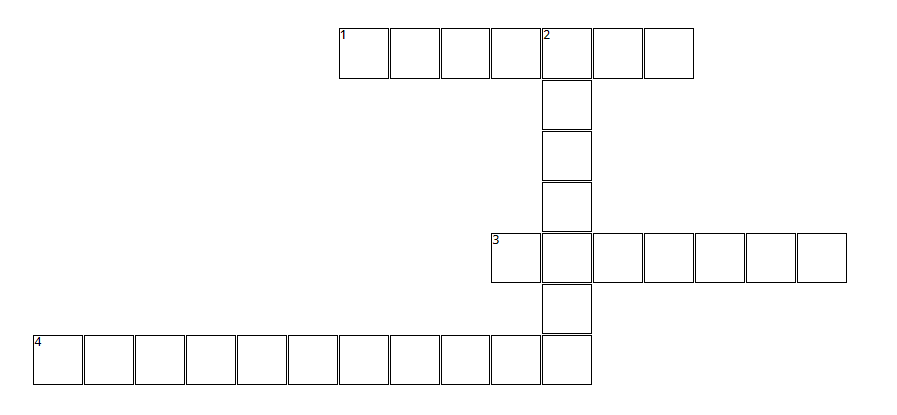
\includegraphics[width=5.33333in,height=4.00000in]{media/image48.png}
%\emph{Siro wajãpi}, 2000. (Reprodução)

%Editora, reproduzir essa imagem. Ela encontra-se presente na página 25,
%do Dossiê 2 -- \emph{Arte Kusiwa} -- Pintura Corporal e Arte Gráfica
%Wajãpi, publicação de 2008 do IPHAN, disponível em:
%http://portal.iphan.gov.br/uploads/publicacao/PatImDos\_PinturaCorporalArteGraficaWajapi\_m.pdf.

\begin{mdframed}[linewidth=2pt,linecolor=salmao]
\coment{
Nesta atividade, cada aluno tem a oportunidade de experimentar uma
criação em artes visuais. Para isso, faz-se necessário que os alunos
tenham acesso a imagem de uma onça-pintada que pode ser apresentada por
meio de projeção ou impressa colorida em papel avulso.

Depois da criação de um padrão gráfico para representar a onça-pintada,
seus alunos podem reproduzir o padrão em folha avulsa para apresentar
aos colegas de turma, explicando porque escolheram aquela(s) cor(es),
aquelas linhas (retas, curvas etc.) aquelas formas (curvas, retas etc.),
entre outras possibilidades.

O resultado desta atividade também pode ser exposto para a comunidade
escolar em espaços da escola.

Saeb: -- Avaliar nas linguagens artísticas a diversidade do patrimônio
cultural da humanidade (material e imaterial), em especial o brasileiro,
a partir de suas diferentes matrizes.

BNCC: (EF15AR25) Conhecer e valorizar o patrimônio cultural, material e
imaterial, de culturas diversas, em especial a brasileira, incluindo-se
suas matrizes indígenas, africanas e europeias, de diferentes épocas,
favorecendo a construção de vocabulário e repertório relativos às
diferentes linguagens artísticas.}
\end{mdframed}

Para responder às atividades 5 e 6, leia o texto de uma notícia.

\begin{quote}
\textbf{Jogo de tabuleiro criado por indígenas empolga estudantes}\\
Em meio a tantas histórias e curiosidades em exposição durante a Semana
Nacional de Ciência e Tecnologia, em Brasília, eram as mesinhas com o
jogo da onça que mais capturavam estudantes de diferentes idades em um
dos estandes montados no pavilhão de eventos do Parque da Cidade.
Atraídos pelo tabuleiro, eles sentavam-se para aprender as regras do
jogo, conhecido pelos indígenas brasileiros antes mesmo da chegada dos
portugueses.

O jogo, disputado em dupla, exige estratégia. Um jogador fica com a onça
e o outro com 14 sementes ou pedrinhas que representam os cachorros. O
jogador com a onça deve capturar cinco cachorros enquanto o oponente
precisa encurralar a onça e impedi-la de se mover pelo tabuleiro. ``Para
não ser cercado, fui pelas beiradas e ganhei dos cachorros'', explicou
David Patrick, 11 anos, aluno do quinto ano da Escola-Classe 407 Norte.
Ele não conhecia o jogo e se divertiu.

``Como o jogo era muito popular em Portugal, acreditava-se que os
portugueses o haviam introduzido no Brasil, mas é um tesouro nacional e
revela o contato dos nossos indígenas com as civilizações mais
desenvolvidas da América pré-colombiana'', explica Zenildo Caetano, 52
anos, professor de educação física do Sesc. Segundo ele, os indígenas
traçavam o tabuleiro no chão e usavam sementes como peças.

\fonte{Disponível em:
\emph{http://portal.mec.gov.br/ultimas-noticias/222-537011943/19235-jogo-de-tabuleiro-criado-por-indigenas-empolga-estudantes}.
Acesso em 22 mar. 2023.}

\num{5} O que podemos afirmar sobre o jogo da onça? Marque a alternativa correta.

\begin{boxlist}
\boxitem{\white{X}} Jogo disputado em equipe.

\boxitem{\white{X}} Jogo de matriz portuguesa.

\boxitem{X} Jogo de matriz indígena.

\boxitem{\white{X}} Jogo de cartas.
\end{boxlist}

\coment{
O jogo da onça, também denominado adugo, é um jogo de tabuleiro popular
entre os povos indígenas Bororo (MT), Manchakeri (AC), Guaranis (SP),
provavelmente de origem inca.

Saeb: -- Avaliar nas linguagens artísticas a diversidade do patrimônio
cultural da humanidade (material e imaterial), em especial o brasileiro,
a partir de suas diferentes matrizes.

BNCC: (EF15AR25) Conhecer e valorizar o patrimônio cultural, material e
imaterial, de culturas diversas, em especial a brasileira, incluindo-se
suas matrizes indígenas, africanas e europeias, de diferentes épocas,
favorecendo a construção de vocabulário e repertório relativos às
diferentes linguagens artísticas.}

\num{6} Siga as instruções e jogue uma ou mais partidas do jogo da onça.

\begin{quote}
\textbf{Jogo da onça}\\
\textbf{Idade recomendada}: a partir dos 6 anos.\\
\textbf{Objetivo do jogo}: a onça precisa capturar 6 cachorros, enquanto
os cachorros precisam imobilizar a onça.\\
\textbf{Materiais}: tabuleiro do jogo (você mesmo pode confeccionar) e
peças para representarem a onça e os cachorros (uma onça e 14
cachorros).\\
\textbf{Número de participantes}: dois.\\
\textbf{Como jogar}: O jogo da onça é um jogo de estratégia, sendo que
os 14 cachorros jogam contra a onça, tentando imobilizá-la, ou seja, não
deixando que ela se movimente. A onça, por sua vez, precisa capturar
cinco cachorros para vencer. Vence aquele que atingir seu objetivo
primeiro.\\
\textbf{Regras}: Os participantes escolhem por conta própria ou a partir
de sorteio quem vai ser a onça e quem vai representar os 14 cachorros. A
peça que representará a onça fica bem no centro do tabuleiro e as
demais, atrás dela, à direita e à esquerda. Veja a imagem do tabuleiro.
\end{quote}


%Editora, redesenhar a imagem, tendo como base a imagem a seguir.
%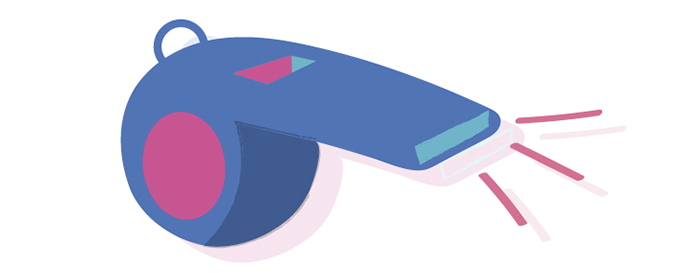
\includegraphics[width=2.92708in,height=3.28779in]{media/image49.png}

Um dos cachorros é quem dá início a partida. Tanto os cães como a onça
podem andar para uma casa vizinha vazia por vez, em qualquer direção. A
onça tentará capturar cinco cachorros da mesma forma que ocorre em um
jogo de dama, ou seja, pulando o cachorro e se dirigindo à próxima casa
vazia. E, como ocorre no jogo de damas também é permitido capturar os
cães em sequência. Já os cachorros não podem capturar a onça, ou melhor,
não podem eliminar sua peça representativa do jogo, mas sim cercá-la por
todos os lados. Dessa maneira, a onça ficará imobilizada e os cachorros
vencem a partida. E, a onça vence quando capturar seis cachorros.

\coment{
Indicamos que, após a leitura do texto Jogo da onça, você assista com
seus alunos os dois vídeos indicados a seguir:

\begin{itemize}
\item
  Vídeo \emph{Jogo da Onça} -- tabuleiro do Suetônio, disponível em:
  \emph{https://www.youtube.com/watch?v=VQwCfAGJt-M}. Acesso em: 22 mar.
  2023. Nesse vídeo, a confecção do tabuleiro é explicada passo a passo,
  além de apresentar a movimentação das peças e os objetivos do
  jogo.

\item
  Vídeo \emph{Jogo da onça} -- aprenda a jogar,
  disponível em: \emph{https://www.youtube.com/watch?v=yE1oDk1-m2E}.
  Acesso em: 22 mar. 2023. Nesse vídeo, algumas estratégias do jogo da
  onça são
  apresentadas.
\end{itemize}

Depois, ajude-os a confeccionar o tabuleiro e a definir as peças
(bolinhas de papel ou massinha, tampinhas, pedras etc.).

E, finalmente, forme duplas para que os alunos possam jogar.

Saeb: -- Avaliar nas linguagens artísticas a diversidade do patrimônio
cultural da humanidade (material e imaterial), em especial o brasileiro,
a partir de suas diferentes matrizes.

BNCC: (EF15AR25) Conhecer e valorizar o patrimônio cultural, material e
imaterial, de culturas diversas, em especial a brasileira, incluindo-se
suas matrizes indígenas, africanas e europeias, de diferentes épocas,
favorecendo a construção de vocabulário e repertório relativos às
diferentes linguagens artísticas.}

\num{7}  Leia o texto.

\begin{quote}
A literatura de cordel é uma manifestação artística que combina vários
elementos, como a escrita, a oralidade e a xilogravura.

Essa expressão cultural brasileira é típica do nordeste do país, mais
precisamente das regiões da Paraíba, Pernambuco, Pará, Alagoas, Rio
Grande do Norte e Ceará.

Esse tipo de literatura se utiliza de folhetos que são tradicionalmente
vendidos em feiras populares.

\textbf{Qual a origem da literatura de cordel?}

A literatura de cordel é uma das heranças lusitanas que herdamos. Ela
surgiu em Portugal por volta do século XII {[}...{]}.

\textbf{A xilogravura no cordel}

Uma das características que se destaca é o uso de desenhos impressos nos
folhetos, que servem para ilustrar as histórias. Esses desenhos são
feitos usando, principalmente, a técnica da xilogravura.

Nesse método, as figuras são feitas a partir do entalhe de uma matriz de
madeira, que recebe uma fina camada de tinta e depois é ``carimbada'' no
papel, transferindo assim o desenho.

As xilogravuras se tornaram uma marca dos folhetos de cordel, e possuem
uma estética bastante própria, com grandes contrastes, formas
simplificadas, uso intenso da cor preta e muitas vezes a presença dos
veios da madeira no resultado final.

\fonte{Disponível em: \emph{https://www.culturagenial.com/literatura-de-cordel/}. Acesso em 22 mar. 2023.}
\end{quote}


Complete o esquema com informações retiradas do texto.

%\textless{}Editora, refazer o esquema.\textgreater{}
%
%\begin{longtable}[]{@{}llllll@{}}
%\toprule
%& & \textbf{Literatura de cordel} & &\tabularnewline
%\midrule
%\endhead
%& & & & &\tabularnewline
%\begin{minipage}[t]{0.16\columnwidth}\raggedright\strut
%\strut
%\end{minipage} & \begin{minipage}[t]{0.16\columnwidth}\raggedright\strut
%\textbf{O que é?}
%
%Manifestação artística que combina a escrita, a oralidade e a
%xilogravura.\strut
%\end{minipage} & \begin{minipage}[t]{0.16\columnwidth}\raggedright\strut
%\strut
%\end{minipage}\tabularnewline
%& & & & &\tabularnewline
%\begin{minipage}[t]{0.16\columnwidth}\raggedright\strut
%\strut
%\end{minipage} & \begin{minipage}[t]{0.16\columnwidth}\raggedright\strut
%\strut
%\end{minipage} & \begin{minipage}[t]{0.16\columnwidth}\raggedright\strut
%\textbf{Qual sua origem/matriz?}
%
%Portugal\strut
%\end{minipage} & \begin{minipage}[t]{0.16\columnwidth}\raggedright\strut
%\strut
%\end{minipage} & \begin{minipage}[t]{0.16\columnwidth}\raggedright\strut
%\strut
%\end{minipage}\tabularnewline
%& & & & &\tabularnewline
%& & \textbf{Xilogravura} & &\tabularnewline
%& & & & &\tabularnewline
%& Figuras feitas a partir do entalhe de uma matriz de madeira, que
%recebe uma fina camada de tinta e depois é "carimbada" no papel,
%transferindo assim o desenho. &\tabularnewline
%& & & & &\tabularnewline
%& & \textbf{Características da técnica} & &\tabularnewline
%& & & & &\tabularnewline
%\begin{minipage}[t]{0.16\columnwidth}\raggedright\strut
%\strut
%\end{minipage} & \begin{minipage}[t]{0.16\columnwidth}\raggedright\strut
%\begin{itemize}
%\item
  %Estética própria
%\item
  %Grandes contrastes
%\item
  %Uso intenso da cor preta
%\item
  %Formas simplificadas
%\end{itemize}\strut
%\end{minipage} & \begin{minipage}[t]{0.16\columnwidth}\raggedright\strut
%\strut
%\end{minipage}\tabularnewline
%\bottomrule
%\end{longtable}

\coment{Indicamos que, após a realização da atividade,
você assista com seus alunos ao vídeo \emph{Xilogravura em isopor
(isogravura)} -- tinta preta, disponível em:
\emph{https://www.youtube.com/watch?v=YTppa6VsuFM}. Acesso em: 22 mar.
2023, para que eles possam aprender a fazer e criar xilogravuras por
meio da técnica ``isogravura'' (xilogravura com isopor).

Para criar as xilogravuras serão necessários os seguintes materiais:
tinta preta, lápis, caneta, bandeja de isopor e papel sulfite.

A seguir, ajude-os a confeccionar uma xilogravura com tema livre. Para
isso, peça a eles para trazer de casa bandejas de isopor.

As xilogravuras criadas por seus alunos podem ser expostas na escola
para a comunidade apreciar.

Saeb: -- Avaliar nas linguagens artísticas a diversidade do patrimônio
cultural da humanidade (material e imaterial), em especial o brasileiro,
a partir de suas diferentes matrizes.

BNCC: (EF15AR25) Conhecer e valorizar o patrimônio cultural, material e
imaterial, de culturas diversas, em especial a brasileira, incluindo-se
suas matrizes indígenas, africanas e europeias, de diferentes épocas,
favorecendo a construção de vocabulário e repertório relativos às
diferentes linguagens artísticas.}

\num{8}  Leia um trecho de uma reportagem.

\textbf{Festa de São João, trazida pelos jesuítas para o Brasil Colônia, atrai multidões hoje}

\textit{Comidas típicas, danças, músicas, fogueiras e fogos das comemorações no
dia 24 de junho mesclam culturas indígenas e africanas. Caruaru e
Campina Grande são estrelas no NE}

{[}...{]}

Trazida para o Brasil pelos jesuítas portugueses durante o período
colonial, a festa de São João adquiriu características próprias. Além
das tradições pagãs e cristãs, temos a incorporação das tradições
indígenas e africanas nas comemorações. {[}...{]}

Em 1808, ao chegar ao Brasil, a Corte portuguesa trouxe consigo vários
hábitos festivos, dando novo vigor às celebrações. Portugal tinha grande
reputação pela beleza dos seus fogos de artifício. Também foram
adaptadas músicas e danças de salão. A mais conhecida delas resiste até
hoje como símbolo da festa, a quadrilha junina. {[}...{]}

Hoje as festas juninas possuem cor local: Caruaru, em Pernambuco, e
Campina Grande, na Paraíba, disputam o título de maior São João do
Mundo. Mas, com maior ou menor destaque, as festas juninas ainda são
realizadas em todas as regiões do Brasil e representam uma das
manifestações culturais mais importantes e ricas, reunindo multidões em
vários estados do país. De acordo com a região, variam os tipos de
dança, indumentária e comida. {[}...{]}

\fonte{Disponível em:
\emph{https://acervo.oglobo.globo.com/em-destaque/festa-de-sao-joao-trazida-pelos-jesuitas-para-brasil-colonia-atrai-multidoes-hoje-19543870}.
Acesso em: 22 mar. 2023.}
\end{quote}

Quais são as matrizes estéticas e culturais da Festa de São João?

\reduline{Europeia (portuguesa), africana e indígena.\hfill}


\coment{Indicamos que, após a primeira leitura do texto pelos alunos,
você releia o último parágrafo do texto e converse com seus eles sobre
as características da Festa junina na comunidade deles. Pergunte: Como
são as danças, a indumentária, as comidas e bebidas? É uma festa de
destaque na comunidade? Entre outras possibilidades de perguntas que
tenham como objetivo refletir sobre as características estéticas e
culturais presentes na
comunidade.

Saeb: -- Avaliar nas linguagens artísticas a diversidade do patrimônio
cultural da humanidade (material e imaterial), em especial o brasileiro,
a partir de suas diferentes matrizes.

BNCC: (EF15AR25) Conhecer e valorizar o patrimônio cultural, material e
imaterial, de culturas diversas, em especial a brasileira, incluindo-se
suas matrizes indígenas, africanas e europeias, de diferentes épocas,
favorecendo a construção de vocabulário e repertório relativos às
diferentes linguagens artísticas.}

\num{9} Leia o texto.

\begin{quote}
\textbf{Artesanato quilombola}\\
Nascido do trabalho dos negros que buscavam a liberdade fugindo das
senzalas, o artesanato quilombola se destaca pelo uso de vários recursos
naturais para a confecção de objetos e instrumentos de trabalho. Alguns
desses materiais são a madeira, a taquara, a palha de milho, a fibra de
bananeira, a canela e a piaçava. Esse artesanato é, então, o resultado
de um rico repertório de bens culturais que expressam os modos
quilombolas de fazer, sentir e se relacionar com a natureza e com a
própria comunidade.

É um trabalho que preserva e promove tanto as técnicas ancestrais quanto
as matérias-primas naturais, disponíveis no ambiente onde vivem e
interagem. Embora o artesanato quilombola tenha se constituído em uma
importante fonte de renda para essas comunidades, a produção artesanal
para a comercialização não é o único fim dessa atividade.

Na vida quilombola, o artesanato tem inúmeras finalidades funcionais,
como a fabricação de utensílios, vestuário e ornamentos para domicílios.
Muitas atividades ajudam na preservação ambiental, como o artesanato com
palha de bananeira ou o de piaçava, usado para fazer vassouras.

Mas o artesanato quilombola também tem propósitos ritualísticos, de
resgate da memória e da cultura histórica das comunidades negras, para
que as gerações mais jovens se reconheçam no coletivo onde estão
inseridas.

\fonte{Disponível em:
\emph{https://www.sebrae.com.br/sites/PortalSebrae/artigos/conheca-o-artesanato-quilombola,0c3a17f4bd962810VgnVCM100000d701210aRCRD}.
Acesso em 22 mar. 2023.}
\end{quote}

Complete o esquema com informações retiradas do texto.

%\textless{}Editora, refazer o esquema.\textgreater{}
%
%\begin{longtable}[]{@{}llllllll@{}}
%\toprule
%& & \textbf{Artesanato quilombola} & &\tabularnewline
%\midrule
%\endhead
%& & & & & & &\tabularnewline
%\begin{minipage}[t]{0.12\columnwidth}\raggedright\strut
%\strut
%\end{minipage} & \begin{minipage}[t]{0.12\columnwidth}\raggedright\strut
%\strut
%\end{minipage} & \begin{minipage}[t]{0.12\columnwidth}\raggedright\strut
%\textbf{Expressão}
%
%Modos quilombolas de fazer, sentir e se relacionar com a natureza e com
%a própria comunidade.\strut
%\end{minipage} & \begin{minipage}[t]{0.12\columnwidth}\raggedright\strut
%\strut
%\end{minipage} & \begin{minipage}[t]{0.12\columnwidth}\raggedright\strut
%\strut
%\end{minipage}\tabularnewline
%& & & & & & &\tabularnewline
%\begin{minipage}[t]{0.12\columnwidth}\raggedright\strut
%\textbf{Recursos naturais}
%
%Madeira, taquara, palha de milho, fibra de bananeira, canela e
%piaçava.\strut
%\end{minipage} & \begin{minipage}[t]{0.12\columnwidth}\raggedright\strut
%\strut
%\end{minipage} & \begin{minipage}[t]{0.12\columnwidth}\raggedright\strut
%\textbf{Finalidade funcional}
%
%Utensílios, vestuário e ornamentos para domicílios.\strut
%\end{minipage} & \begin{minipage}[t]{0.12\columnwidth}\raggedright\strut
%\strut
%\end{minipage} & \begin{minipage}[t]{0.12\columnwidth}\raggedright\strut
%\textbf{Outras finalidades}
%
%Ritualísticas, de resgate da memória e da cultura histórica das
%comunidades negras, para que as gerações mais jovens se reconheçam no
%coletivo onde estão inseridas.\strut
%\end{minipage}\tabularnewline
%\bottomrule
%\end{longtable}

\coment{Indicamos que a primeira leitura seja feita por você, com
pausas em cada parágrafo, para discutir os aspectos abordados e auxiliar
na compreensão deles.

Depois, solicite que os alunos façam uma leitura individual
para verificar se ainda restam dúvidas. Se elas existirem, auxilie-os na
compreensão e a seguir, peça que realizem a atividade, completando o
esquema com informações retiradas do
texto.

Para enriquecer as experiências dos alunos
sobre comunidades quilombolas, sugerimos que assista, junto com eles, ao
vídeo Ep. 02 \textbar{} \emph{O Artesanato do Quilombo}, disponível
em: \emph{https://www.youtube.com/watch?v=sNAy5aY1Wi0}. Acesso em: 22 mar.
2023. Nele encontra-se em destaque a produção artesanal da Comunidade
Quilombola de Massarandupió, na Bahia, passada de geração em geração,
demonstrando a união da comunidade e os cuidados com o meio ambiente.

Saeb: -- Avaliar nas linguagens artísticas a diversidade do patrimônio
cultural da humanidade (material e imaterial), em especial o brasileiro,
a partir de suas diferentes matrizes.

BNCC: (EF15AR25) Conhecer e valorizar o patrimônio cultural, material e
imaterial, de culturas diversas, em especial a brasileira, incluindo-se
suas matrizes indígenas, africanas e europeias, de diferentes épocas,
favorecendo a construção de vocabulário e repertório relativos às
diferentes linguagens artísticas.}

\num{10} Leia o texto.
%
%\begin{longtable}[]{@{}l@{}}
%\toprule
%\begin{minipage}[b]{0.97\columnwidth}\raggedright\strut
%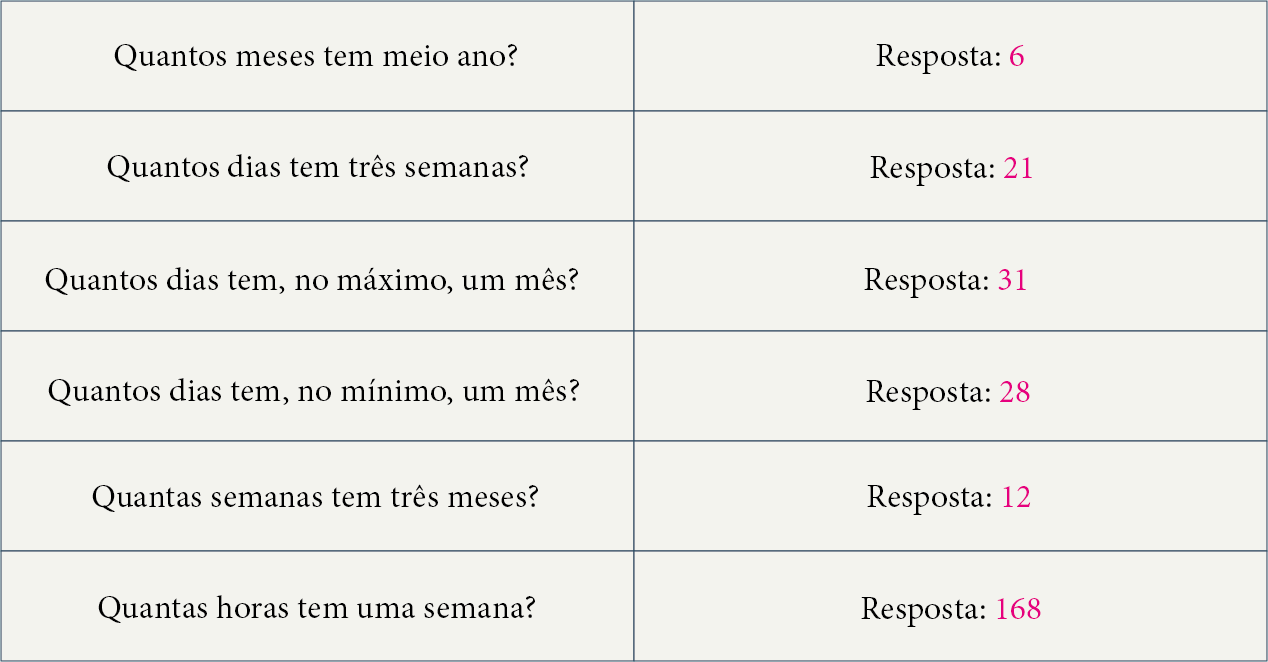
\includegraphics[width=2.22353in,height=1.66667in]{media/image50.png}

%Instrumentos utilizados no Tambor de Crioula: tambor grande, meião e crivador.
%\emph{https://commons.wikimedia.org/wiki/File:Casa_do_Tambor_de_Crioula_-_06.jpg}

\begin{quote}
Essa manifestação afro-brasileira ocorre na maioria dos municípios do
Maranhão, envolvendo uma dança circular feminina, canto e percussão de
tambores. Dela participam as coreiras ou dançadeiras, conduzidas pelo
ritmo intenso dos tambores e pelo influxo das toadas evocadas por
tocadores e cantadores, culminando na punga ou umbigada -- gesto
característico, entendido como saudação e convite.

\fonte{Disponível em: \emph{https://www.palmares.gov.br/?p=37269}. Acesso em: 22
mar. 2023.}
\end{quote}

Defina o patrimônio imaterial Tambor de Crioula do Maranhão.

\reduline{É uma forma de expressão de matriz afro-brasileira que envolve dança
circular, canto e percussão de tambores. É realizado sem local
específico ou calendário pré-fixado.\hfill}

\coment{
Para enriquecer as experiências dos alunos com percussão de instrumentos
e produção de sons, indicamos que eles construam um tambor com balde e
uma baqueta seguindo as instruções de como fazer. Para isso, sugerimos
que assista, junto com eles, ao vídeo \emph{Como fazer um tambor com um
balde}, disponível em:
\emph{https://www.youtube.com/watch?v=22IagIwP3Jc}. Acesso em: 22 mar.
2023, que descreve de forma simples como fazer um tambor e uma baqueta,
quais materiais são necessários e indica ritmos distintos para a prática
das batidas no tambor.

Saeb: -- Avaliar nas linguagens artísticas a diversidade do patrimônio
cultural da humanidade (material e imaterial), em especial o brasileiro,
a partir de suas diferentes matrizes.

BNCC: (EF15AR25) Conhecer e valorizar o patrimônio cultural, material e
imaterial, de culturas diversas, em especial a brasileira, incluindo-se
suas matrizes indígenas, africanas e europeias, de diferentes épocas,
favorecendo a construção de vocabulário e repertório relativos às
diferentes linguagens artísticas.}

\colorsec{Treino}

\num{1}  Leia o texto.

\begin{quote}
Para acalentar seus filhos durante as terríveis viagens a bordo dos
tumbeiros -- navio de pequeno porte que realizava o transporte de
escravizados entre África e Brasil -- as mães africanas rasgavam
retalhos de suas saias e a partir deles criavam pequenas bonecas, feitas
de tranças ou nós, que serviam como amuleto de proteção. As bonecas,
símbolo de resistência, ficaram conhecidas como \emph{abayomi}, termo
que significa ``encontro precioso'', em iorubá, uma das maiores etnias
do continente africano cuja população habita parte da Nigéria, Benin,
Togo e Costa do Marfim.

\fonte{Disponível em:
\emph{http://www.afreaka.com.br/notas/bonecas-abayomi-simbolo-de-resistencia-tradicao-e-poder-feminino/}.
Acesso em: 22 mar. 2023.}
\end{quote}

A partir da descrição feita pelo texto, assinale a alternativa que
contém imagem de boneca abayomi.
%
%Editora, seria interessante retirar os fundos das imagens,
%padronizando-os. Acredito que um fundo branco, seria interessante.
%
%a)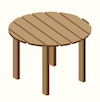
\includegraphics[width=2.20680in,height=2.19792in]{media/image51.png}
%\emph{https://live.staticflickr.com/8687/16615164110_b2c6be7252.jpg}
%
%b)\emph{https://commons.wikimedia.org/wiki/File:Doll_(CH_18188797).jpg?uselang=pt}
%
%c)\emph{https://commons.wikimedia.org/wiki/File:Boneca_de_pano_MN_01.jpg?uselang=pt}
%
%d)\emph{https://commons.wikimedia.org/wiki/File:GarifunaDolls.JPG?uselang=pt}
%
%Editora, retirar o fundo da imagem, deixando apenas os
%bonecos a mostra.

\coment{
Nível: fácil.

Saeb: -- Avaliar nas linguagens artísticas a diversidade do patrimônio
cultural da humanidade (material e imaterial), em especial o brasileiro,
a partir de suas diferentes matrizes.

BNCC: (EF15AR25) Conhecer e valorizar o patrimônio cultural, material e
imaterial, de culturas diversas, em especial a brasileira, incluindo-se
suas matrizes indígenas, africanas e europeias, de diferentes épocas,
favorecendo a construção de vocabulário e repertório relativos às
diferentes linguagens artísticas.

Resposta:

a) Correta. As bonecas apresentadas na imagem foram feitas com retalhos
de tecido, apresentam nós na sua confecção e foram feitas sem costura.
Além disso, nas bonecas abayomi, em sua origem, não havia a
possibilidade de demarcação de olho, nariz nem boca.
b) Incorreta. Trata-se de uma boneca feita de retalhos de pano, mas onde
a tecnologia da costura se faz presente.
c) Incorreta. É uma boneca feita com retalhos de pano, com vestimenta
complexa, colares de contas, pulseiras e onde a tecnologia da costura se
faz presente.
d) Incorreta. São bonecos de pano feitos com retalhos de tecidos, seus
corpos e vestimentas foram costurados.}

\num{2}  Assinale a alternativa cuja descrição corresponde a um patrimônio imaterial.

\begin{escolha}
\item
  A cidade de Ouro Preto e a primeira cidade brasileira a receber o
  título de Patrimônio Mundial, conferido pela Unesco, em 1980. Seu
  traçado urbano colonial mantém-se intacto e o mesmo ocorre com os
  exemplares da arquitetura religiosa e civil, e as suas obras de arte
  preservadas. (Fonte: IPHAN)
\item
  O Parque Estadual Veredas do Peruaçu, situado no município de Cônego
  Marinho (MG), abriga um complexo de veredas e lagoas, dentre as quais
  está a vereda do Peruaçu (que significa gruta grande) que dá nome ao
  parque. (Fonte: IPHAN)
\item
  Os mestres de capoeira são detentores dos conhecimentos tradicionais
  da manifestação Roda de Capoeira e responsáveis pela transmissão de
  suas práticas, rituais e herança cultural. (Fonte: IPHAN)
\item
  A Igreja Matriz de Nossa Senhora da Conceição, construção do século
  XVIII, destaca-se pelo suporte arquitetônico e por seu interior. O
  frontispício, com seu belo pórtico esculpido é obra do Aleijadinho.
  (Fonte: IPHAN)
\end{escolha}


\coment{
Nível: médio.

Saeb: -- Avaliar nas linguagens artísticas a diversidade do patrimônio
cultural da humanidade (material e imaterial), em especial o brasileiro,
a partir de suas diferentes matrizes.

BNCC: (EF15AR25) Conhecer e valorizar o patrimônio cultural, material e
imaterial, de culturas diversas, em especial a brasileira, incluindo-se
suas matrizes indígenas, africanas e europeias, de diferentes épocas,
favorecendo a construção de vocabulário e repertório relativos às
diferentes linguagens artísticas.

a)  Incorreta. A cidade de Ouro Preto (MG) é um bem de natureza material.
  Os bens de natureza material podem ser imóveis como as cidades
  históricas.
b) Incorreta. O Parque Estadual Veredas do Peruaçu (MG) é um bem imóvel
  e, por isso, de natureza material. Trata-se de um monumento natural,
  constituído por formações físicas e biológicas, detentor de valor do
  ponto de vista estético e científico.
c) Correta. Os conhecimentos, as técnicas e práticas se constituem
  patrimônios imateriais. Mestres de capoeira é um ofício e, por isso,
  se enquadra na classificação de bem imaterial.
d) Incorreta. A Matriz de Nossa Senhora da Conceição é um bem imóvel, ou
  seja, de natureza material.}

\num{3}  Assinale a alternativa que corresponde a uma característica do
  patrimônio cultural brasileiro literatura de cordel.

\begin{escolha}
\item
  Gênero literário em prosa.
\item
  Temas populares da cultura africana.
\item
  Literatura de tradição regional.
\item
  Linguagem culta (formal).
\end{escolha}

\coment{Nível: difícil.

Saeb: -- Avaliar nas linguagens artísticas a diversidade do patrimônio
cultural da humanidade (material e imaterial), em especial o brasileiro,
a partir de suas diferentes matrizes.

BNCC: (EF15AR25) Conhecer e valorizar o patrimônio cultural, material e
imaterial, de culturas diversas, em especial a brasileira, incluindo-se
suas matrizes indígenas, africanas e europeias, de diferentes épocas,
favorecendo a construção de vocabulário e repertório relativos às
diferentes linguagens artísticas.

a) Incorreta. É um gênero literário em verso.
b) Incorreta. A literatura de cordel possui uma variedade de temas
  populares e da cultura nacional.
c) Correta. Apesar de ser apreciada e ter representantes em todo o
  Brasil, a literatura de cordel é de tradição nordestina.
d) Incorreta. A linguagem da literatura de cordel é popular, oral e
  informal.}




\chapter{Simulado 1}

\num{1}  Observe a imagem.

%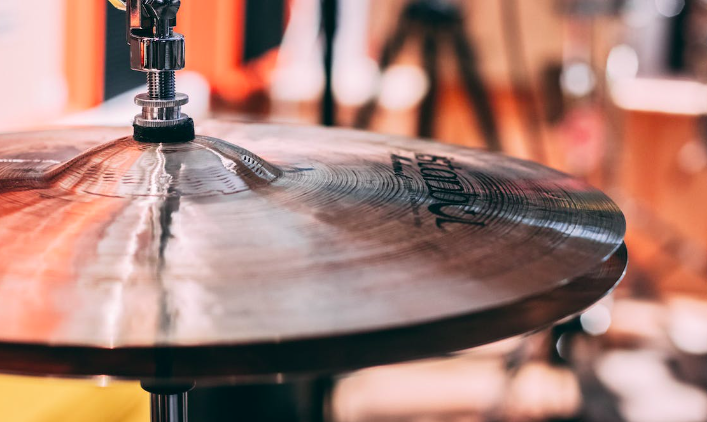
\includegraphics[width=5.90625in,height=3.86458in]{media/image1.png}

Pinturas rupestres no Parque Nacional Serra da Capivara,
declarado Patrimônio Mundial pela UNESCO em vista de sua importância
arqueológica.
%\emph{https://commons.wikimedia.org/wiki/File:Serra_da_Capivara_-_Several_Paintings_2b.jpg}

Assinale a alternativa que contém uma característica desta manifestação
artística.

\begin{escolha}
\item
  As figuras são percebidas através de três dimensões: altura,
  profundidade e largura.
\item
  Representa as imagens em relevo.
\item
  Arte tridimensional de importância arqueológica.
\item
  Apresenta figuras dispostas em superfície plana.
\end{escolha}

\coment{Nível: difícil.

a)  Incorreta. A pintura apresenta duas dimensões: altura e largura.
b)  Incorreta. O relevo é uma característica de obras tridimensionais.
c)  Incorreta. É um exemplo de arte bidimensional.
d)  Correta. Por se tratar de uma arte dimensional, apresenta como
  característica a superfície plana.

Saeb: -- Reconhecer elementos constitutivos das artes visuais, dança,
música e teatro.

BNCC: (EF15AR02) Explorar e reconhecer elementos constitutivos das artes
visuais (ponto, linha, forma, cor, espaço, movimento etc.).}

\num{2}  Assinale a alternativa que apresenta o nome da manifestação artística
  cujo responsável pela ação é o ator.

\begin{escolha}
\item
  Dança.
\item
  Escultura.
\item
  Teatro.
\item
  Artesanato.
\end{escolha}

\coment{Nível: fácil.

a)  Incorreta. Na dança o responsável pela ação é o dançarino.
b)  Incorreta. Na escultura o responsável pela ação é o artista plástico.
c)  Correta. No teatro o responsável pela ação é o ator.
d)  Incorreta. No artesanato o responsável pela ação é o artesão.

Saeb: -- Identificar características do sistema de circulação das artes
visuais, dança, música e teatro em diferentes contextos (teatros,
palcos, museus, galerias, artistas, artesãos, curadores, produtores
etc.).

BNCC: (EF15AR01) Identificar e apreciar formas distintas das artes
visuais tradicionais e contemporâneas, cultivando a percepção, o
imaginário, a capacidade de simbolizar e o repertório imagético.}

\num{3}  Observe a imagem.

%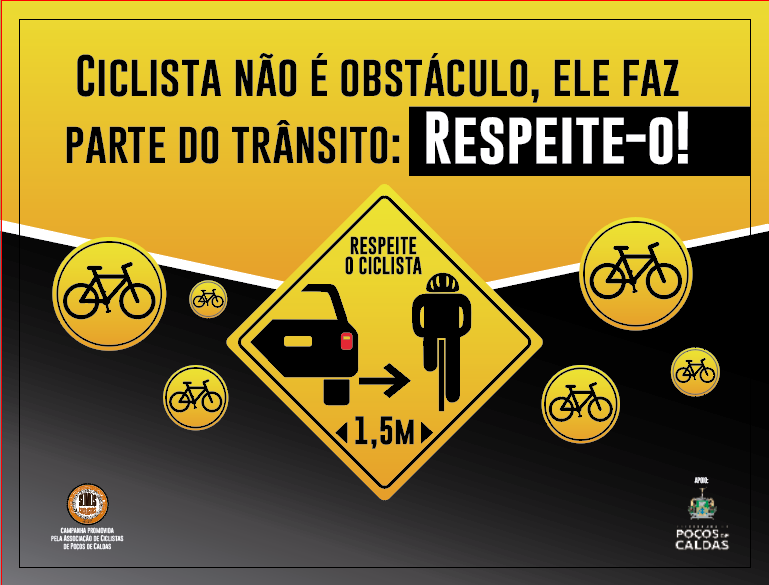
\includegraphics[width=4.12074in,height=2.70833in]{media/image2.png}

Dança em frente ao tronco. Festa do Kuarup, na aldeia Kamayurá, Alto Xingu (MT).

%\emph{https://commons.wikimedia.org/wiki/File:Festa_do_Kuarup_dan\%C3\%A7a_em_torno_do_tronco.jpg}

Assinale a alternativa que corresponde à característica da dança da Festa do Kuarup.

\begin{escolha}
\item
  É uma manifestação artística que tem a expressão relacionada ao
  sentido da visão.
\item
  É uma manifestação artística que tem o corpo como instrumento de
  expressão.
\item
  É uma manifestação artística que tem o som como meio de expressão.
\item
  É uma manifestação artística que reúne três elementos básicos: o(s)
  ator(es), o texto e o público.
\end{escolha}

\coment{Nível: médio.

a) Incorreta. São nas artes visuais que a manifestação artística tem a
  expressão relacionada ao sentido da visão.
b) Correta. É na dança que a manifestação artística tem o corpo como
  instrumento de expressão.
c) Incorreta. É na música que a manifestação artística tem o som como
  meio de expressão.
d) Incorreta. É no teatro que a manifestação artística reúne três
  elementos básicos: o(s) ator(es), o texto e o público.

Saeb: -- Reconhecer elementos constitutivos das artes visuais, dança,
música e teatro.

BNCC: (EF15AR08) Experimentar e apreciar formas distintas de
manifestações da dança presentes em diferentes contextos, cultivando a
percepção, o imaginário, a capacidade de simbolizar e o repertório
corporal.}

\chapter{Simulado 2}

\num{1}  Leia o texto.
%Afoxé.

%\emph{https://commons.wikimedia.org/wiki/File:Abe_agbe_afoxe.jpg} (Esse link corresponde apenas à imagem.)

O afoxé (instrumento musical) é composto por uma cabaça coberta por uma
rede formada por sementes, miçangas ou contas. O som desse instrumento é
produzido quando se gira a rede em um sentido e a base do instrumento (a
cabaça) no sentido oposto.

Assinale a alternativa que corresponde à forma como o som do afoxé é
produzido.

\begin{escolha}
\item
  Produz som pela vibração do instrumento.
\item
  Produz som pela vibração de cordas.
\item
  Produz som pela vibração de uma membrana esticada em algum suporte.
\item
  Produz som pela vibração do ar no seu interior.
\end{escolha}

\coment{Nível: fácil.

Saeb: -- Identificar as características de instrumentos musicais
variados, bem como o potencial musical do corpo humano.

Resposta:

a) Correta. O afoxé é um instrumento musical classificado como idiofone,
ou seja, que produz som através da vibração de seu próprio corpo.
b) Incorreta. Os instrumentos musicais que produzem som através da
vibração das cordas são os cordofones. Exemplo: violão.
c) Incorreta. Os instrumentos musicais que produzem som por meio de uma
membrana são os membrafones. Exemplo: tamborim.
d) Incorreta. Os instrumentos que produzem som através da vibração do ar
são os aerofones. Exemplo: trombone.}

\num{2}  Leia o texto.

\begin{quote}
A ``arte afro-brasileira'' é antes de mais nada contemporânea: ganhou
nome no século XX e passou a ser reconhecida como qualquer manifestação
plástica e visual que retome, de um lado, a \emph{estética} e
a \emph{religiosidade} africanas tradicionais e, de outro,
os \emph{cenários socioculturais do negro} no Brasil.

\fonte{Disponível em:
\emph{https://www.institutotomieohtake.org.br/o\_instituto/interna/exposiasames-e-crasticos-de-arte-afro-brasileira-um-conceito-em-disputa\#:~:text=a\%20\%E2\%80\%9Carte\%20afro\%2Dbrasileira\%E2\%80\%9D,socioculturais\%20do\%20negro\%20no\%20Brasil}.
Acesso em: 25 mar. 2023.}
\end{quote}

Assinale a alternativa que contém um exemplo de arte afro-brasileira.

%\begin{longtable}[]{@{}l@{}}
%\toprule
%\begin{minipage}[b]{0.97\columnwidth}\raggedright\strut
%\begin{escolha}
%\item
%\end{escolha}
%
%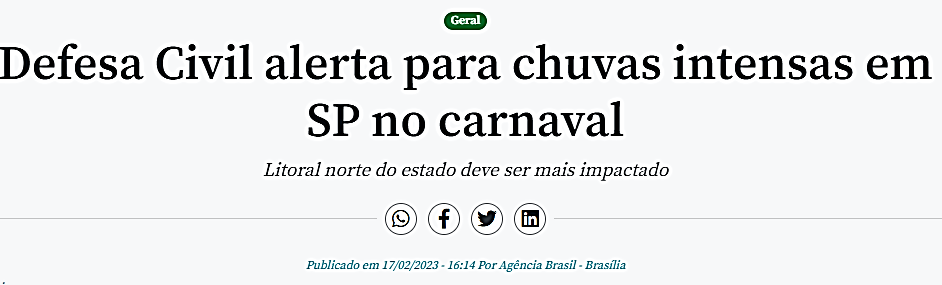
\includegraphics[width=1.37789in,height=1.37500in]{media/image4.png}
%
%Máscara dos yakas, grupo étnico de Angola. Museu Afro Brasil.
%
%\emph{https://commons.wikimedia.org/wiki/File:M\%C3\%A1scara_(povo_yaka)_(01).jpg}\strut
%\end{minipage}\tabularnewline
%\midrule
%\endhead
%\begin{minipage}[t]{0.97\columnwidth}\raggedright\strut
%b)
%
%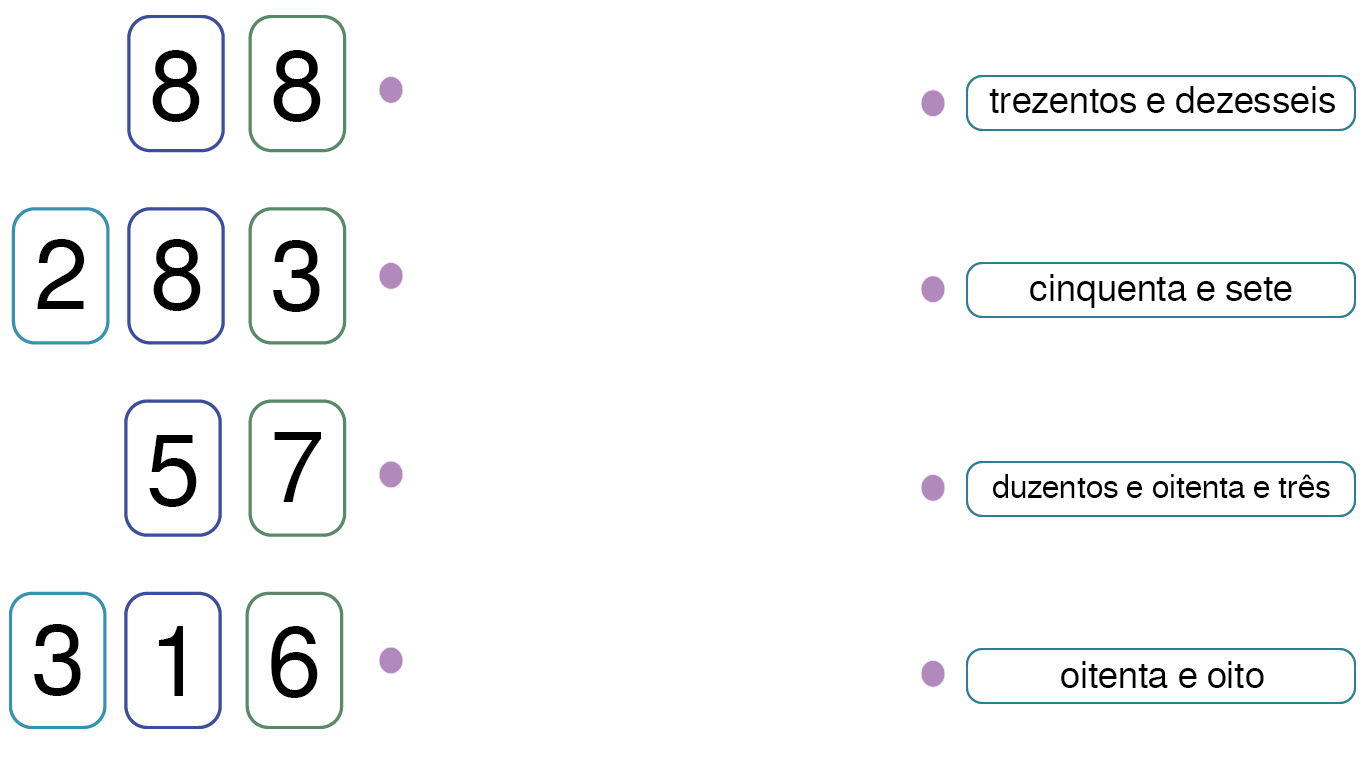
\includegraphics[width=2.73958in,height=1.83446in]{media/image5.png}
%
%Cortejo de maracatu. Recife, Brasil.
%
%\emph{https://commons.wikimedia.org/wiki/File:Encontro_estadual_de_maracatus.jpg}\strut
%\end{minipage}\tabularnewline
%\begin{minipage}[t]{0.97\columnwidth}\raggedright\strut
%c)
%
%Painel de porta (1910-1914), povo iorubá, Nigéria, África.
%
%\emph{https://commons.wikimedia.org/wiki/File:Pair_of_door_panels_and_lintel_Yoruba_BM.jpg?uselang=pt}\strut
%\end{minipage}\tabularnewline
%\begin{minipage}[t]{0.97\columnwidth}\raggedright\strut
%d)
%
%Escultura yumbe, da República Democrática do Congo, África.
%
%\emph{https://commons.wikimedia.org/wiki/File:African_Art,_Yombe_sculpture,_Louvre.jpg}\strut
%\end{minipage}\tabularnewline
%\bottomrule
%\end{longtable}

\coment{Nível: difícil.

Saeb: -- Reconhecer a influência de distintas matrizes estéticas e
culturais nas manifestações das artes visuais, dança, música e teatro na
cultura brasileira.

BNCC: (EF15AR03) Reconhecer e analisar a influência de distintas
matrizes estéticas e culturais das artes visuais nas manifestações
artísticas das culturas locais, regionais e nacionais.

a) Incorreta. A máscara dos yakas, apesar de fazer parte do acervo do
Museu Afro Brasil, apresenta estética de matriz africana, mas faz parte
do contexto sociocultural do negro na África.
b) Correta. O maracatu é uma manifestação cultural afro-brasileira que
apresenta elementos estéticos de matriz africana e que surgiu no estado
de Pernambuco, no século XVIII, no contexto sociocultural do período
colonial brasileiro.
c) Incorreta. O painel de porta do povo iorubá apresenta estética de
matriz africana, mas faz parte do contexto sociocultural do negro na
África.
d) Incorreta. A escultura yumbe apresenta estética de matriz africana,
mas faz parte do contexto sociocultural do negro na África.}

\num{3} Assinale a alternativa que apresenta movimento corporal próprio das danças do hip-hop.

%\begin{longtable}[]{@{}l@{}}
%\toprule
%\begin{minipage}[b]{0.97\columnwidth}\raggedright\strut
%\begin{escolha}
%\item
%\end{escolha}
%
%Editora, borrar as referências de marcas na imagem.
%
%\emph{https://live.staticflickr.com/4069/4438178315_7d9c4cdea2_b.jpg}\strut
%\end{minipage}\tabularnewline
%\midrule
%\endhead
%\begin{minipage}[t]{0.97\columnwidth}\raggedright\strut
%b)
%
%Editora, borrar o texto da faixa.
%
%\emph{https://live.staticflickr.com/2800/4345161183_4cf633fd9b_b.jpg}\strut
%\end{minipage}\tabularnewline
%\begin{minipage}[t]{0.97\columnwidth}\raggedright\strut
%c)
%
%Editora, borrar as referências de marcas na imagem.
%
%\emph{https://commons.wikimedia.org/wiki/File:Thai_Breakdancers.jpg}\strut
%\end{minipage}\tabularnewline
%\begin{minipage}[t]{0.97\columnwidth}\raggedright\strut
%d)
%
%\emph{https://commons.wikimedia.org/wiki/File:Chica_haciendo_posiciones_de_ballet.jpg?uselang=pt}\strut
%\end{minipage}\tabularnewline
%\bottomrule
%\end{longtable}

\coment{Nível: médio.

Saeb: -- Analisar relações entre as partes corporais e seu todo na
estética da dança.

Resposta:

a) Incorreta. Movimento corporal característico da dança do frevo.
b) Incorreta. Movimento corporal característico da dança do tango.
c) Correta. Movimento corporal característico da estética da dança hip
hop. Movimento \emph{power move} (pernas para cima, cabeça para baixo,
tendo como apoio as mãos, cabeças ou ombros).
d) Incorreta. Movimento característico da dança balé.}

\chapter{Simulado 3}

\num{1}  Leia o texto.

%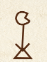
\includegraphics[width=2.64583in,height=2.04387in]{media/image12.png}
%\emph{https://commons.wikimedia.org/wiki/File:Luta_indigena.jpg}\strut

\begin{quote}
Com enfeites de linha, plumas e miçangas e o corpo pintado de jenipapo e
urucum, os guerreiros são convocados para o embate.

Frente a frente, e abaixados para protegerem as pernas, os oponentes
giram em forma circular e se enfrentam primeiro pelo olhar.
Posteriormente, agarram-se para ver quem consegue levantar o adversário
e levá-lo ao chão, encostando as costas no solo ou, ainda, tocar-lhe a
parte inferior do joelho, casos em que se finaliza a luta. {[}...{]}

\fonte{Disponível em:
\emph{https://www.gov.br/funai/pt-br/assuntos/noticias/2022-02/huka-huka-a-luta-corporal-do-xingu-contribui-para-manter-viva-a-cultura-indigena-no-mato-grosso}.
Acesso em: 26 mar. 2023. (Adaptado para fins didáticos.)}
\end{quote}

Assinale a alternativa que corresponde às características da
manifestação cultural huka-huka.

\begin{escolha}
\item
  Patrimônio cultural imaterial de matriz indígena.
\item
  Patrimônio cultural material de matriz indígena.
\item
  Patrimônio cultural material transmitido de geração a geração.
\item
  Patrimônio cultural imaterial dos povos indígenas do nordeste
  brasileiro.
\end{escolha}

\coment{Nível: médio.

Saeb: -- Avaliar nas linguagens artísticas a diversidade do patrimônio
cultural da humanidade (material e imaterial), em especial o brasileiro,
a partir de suas diferentes matrizes.

BNCC: (EF15AR25) Conhecer e valorizar o patrimônio cultural, material e
imaterial, de culturas diversas, em especial a brasileira, incluindo-se
suas matrizes indígenas, africanas e europeias, de diferentes épocas,
favorecendo a construção de vocabulário e repertório relativos às
diferentes linguagens artísticas.

a) Correta. É um patrimônio imaterial, pois diz respeito a práticas e
domínios da vida social dos povos indígenas do Xingu.
b) Incorreta. É um patrimônio imaterial.
c) Incorreta. É transmitido de geração a geração, mas é um patrimônio
imaterial.
d) Incorreta. É um patrimônio cultural imaterial, mas pertence ao
patrimônio de povos indígenas do centro-oeste brasileiro (Mato Grosso do
Sul).}

\num{2}  Leia o texto.

\begin{quote}
Um dos principais símbolos da cultura nordestina, o forró é uma
manifestação artística de diferentes significados {[}...{]}, podendo
servir tanto para definir um ritmo musical, o estilo de dança e até a
festividade em que ele acontece {[}...{]}.

Para que uma expressão artística se configure como forró é necessário
que uma sequência de ritmos nordestinos esteja presente, como o xaxado,
coco, baião, xote, dentre outros.

%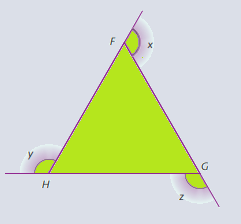
\includegraphics[width=2.15970in,height=1.42708in]{media/image13.png}
%Típico grupo de forró com acordeão, triângulo e zabumba.
%\emph{https://commons.wikimedia.org/wiki/File:Forrozeiros_(9290035008).jpg}

Também é característica a presença sonora de instrumentos como zabumba,
triângulo e sanfona, assim como a representação da dança entre casais,
com os corpos colados e arrastando os pés no chão. {[}...{]}

\fonte{Disponível em: \emph{https://www.sabra.org.br/site/forro-nordeste/}.
Acesso em: 26 mar. 2023.}
\end{quote}

Marque a alternativa que corresponde às linguagens artísticas presentes
no forró.

\begin{escolha}
\item
  Artes visuais e dança.
\item
  Artes visuais e música.
\item
  Dança e música.
\item
  Música e teatro.
\end{escolha}

\coment{Nível: fácil.

Saeb: -- Avaliar nas linguagens artísticas a diversidade do patrimônio
cultural da humanidade (material e imaterial), em especial o brasileiro,
a partir de suas diferentes matrizes.

BNCC: (EF15AR25) Conhecer e valorizar o patrimônio cultural, material e
imaterial, de culturas diversas, em especial a brasileira, incluindo-se
suas matrizes indígenas, africanas e europeias, de diferentes épocas,
favorecendo a construção de vocabulário e repertório relativos às
diferentes linguagens artísticas.

a) Incorreta. A dança é uma linguagem artística representativa do forró,
mas a linguagem das artes visuais não se faz presente no forró.
b) Incorreta. A música é uma linguagem artística presente no forró,
porém a linguagem das artes visuais não se encontra representada nesta
manifestação artística.
c) Correta. A dança e a música são linguagens artísticas presentes no
forró.
d) Incorreta. A música é uma linguagem representativa do forró, mas a
linguagem do teatro não é característica desta manifestação cultural.}

\num{3}  Observe a imagem de um exemplo de cestaria confeccionada pelos
  indígenas yanomamis.

%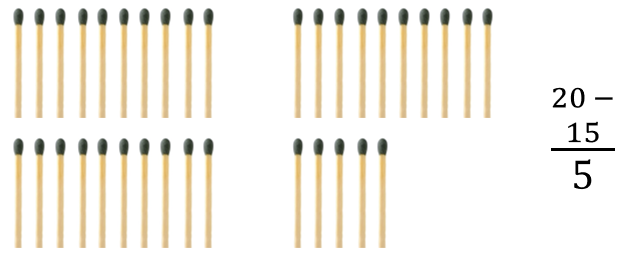
\includegraphics[width=3.00000in,height=2.38624in]{media/image14.png}
%Mulher yanomami.
%\emph{https://commons.wikimedia.org/wiki/File:Eduardo_Jun_1999_1.jpg}

Assinale a alternativa que contém a descrição do tipo de cesto correspondente à imagem.

\begin{escolha}
\item
  O cesto \emph{Wɨɨ a} é um cesto alongado com fundo arredondado e ponto
  fechado. São trançados por mulheres e feitos de cipó titica com
  detalhes de fios de fungo negro ou com pinturas de tintas naturais
  como o urucum. {[}...{]}
\item
  O balaio \emph{Soteha} é confeccionado por homens Yanomami do grupo
  Sanöma. {[}...{]} Esse cesto tem bordas baixas e é trançado com fibras
  de arumã em cor crua e fibras tingidas com tintas naturais. Serve para
  apoiar frutas e outros alimentos, recolher a massa de mandioca,
  guardar e servir o beiju e o que é comido coletivamente em família.
\item
  O \emph{Xotehe} é um cesto raso trançado de cipó titica com fios de
  fungo negro ou tiras de raízes pretas da palmeira paxiubinha. É feito
  por mulheres e é objeto de uso diário nas comunidades. São utilizados
  para acondicionar alimentos, algodão e pequenos objetos.
\item
  O \emph{Kotomasö} é um cesto tubular trançado com fibras de arumã em
  cor crua e fibras tingidas com tintas naturais. Esse utensílio
  culinário é confeccionado pelos homens Yanomami e utilizado pelas
  mulheres para espremer o suco venenoso da mandioca brava. {[}...{]}
\end{escolha}

\fonte{Disponível em:
\emph{https://www.origensbrasil.org.br/produto.php?qrcode=5311\#: :text=Cada\%20objeto\%20produzido\%20pelo\%20povo,ro\%C3\%A7as\%20e\%20\%C3\%A1rea\%20de\%20ca\%C3\%A7a}.
Acesso em: 26 mar. 2023.}

\coment{Nível: difícil.

Saeb: -- Avaliar nas linguagens artísticas a diversidade do patrimônio
cultural da humanidade (material e imaterial), em especial o brasileiro,
a partir de suas diferentes matrizes.

BNCC: (EF15AR25) Conhecer e valorizar o patrimônio cultural, material e
imaterial, de culturas diversas, em especial a brasileira, incluindo-se
suas matrizes indígenas, africanas e europeias, de diferentes épocas,
favorecendo a construção de vocabulário e repertório relativos às
diferentes linguagens artísticas.

a) Incorreta. Apesar do cesto \emph{Wɨɨ a} ser confeccionado por
mulheres a imagem mostra um cesto raso e não alongado.
b) Incorreta. O balaio \emph{Soteha} é confeccionado por homens Yanomami
e a imagem mostra uma mulher confecionando.
c) Correta. O \emph{Xotehe} é um cesto raso confeccionado por mulheres.
d) Incorreta. O \emph{Kotomasö} é um cesto tubular confeccionado por
homens.}

\chapter{Simulado 4}

\num{1}  Observe a fotografia.

%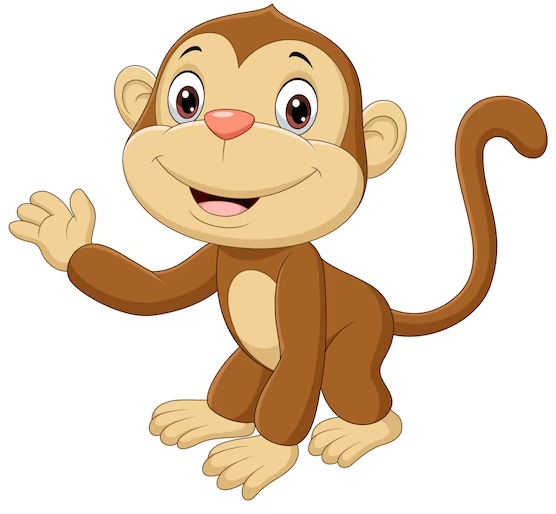
\includegraphics[width=5.90625in,height=3.40625in]{media/image15.png}
%Improvisação de contato na dança.
%\emph{https://cdn.pixabay.com/photo/2018/09/17/19/59/contact-improvisation-3684693_960_720.jpg}

A improvisação é uma característica da dança contemporânea. Assinale a
alternativa que contém outra característica deste gênero de dança.

\begin{escolha}
\item
  Possui técnica e vocabulário próprio.
\item
  Não existem limitações de movimentos.
\item
  Roupas e acessórios padronizados.
\item
  Postura ereta e verticalizada.
\end{escolha}

\coment{Nível: difícil.

a) Incorreta. O balé clássico é um gênero de dança que possui técnica e
  vocabulário próprio. Na dança contemporânea não existem técnicas, nem
  vocabulário predefinidos.
b) Correta. A dança contemporânea não se define em movimentos específicos
  e o bailarino/intérprete tem autonomia para construir sua coreografia.
c) Incorreta. Na dança contemporânea não há limitações para roupas e
  acessórios, inexistindo um padrão.
d) Incorreta. A postura reta e verticalizada é uma característica do balé
  clássico. A dança contemporânea tem como uma de suas características a
  maior mobilidade da coluna.

Saeb: -- Identificar distintas formas e/ou gêneros de expressão da dança,
da música e do teatro em diferentes contextos e práticas.

BNCC: (EF15AR08) Experimentar e apreciar formas distintas de
manifestações da dança presentes em diferentes contextos, cultivando a
percepção, o imaginário, a capacidade de simbolizar e o repertório
corporal.}

\num{2}  Leia a descrição de um instrumento musical.

\begin{quote}
Um dos mais importantes instrumentos musicais brasileiros, chegou por
aqui com os escravizados de Angola e é um dos principais elementos de
uma roda de capoeira.

{[}...{]} É importante para a capoeira, visto que controla o ritmo da
roda.

\fonte{Disponível em:
\emph{https://www.sabra.org.br/site/instrumentos-musicais-2/}. Acesso em:
21 mar. 2023. (Adaptação para fins didáticos.)}
\end{quote}

Assinale a alternativa que corresponde à descrição.

\begin{escolha}
\item
  Pandeiro.
\item
  Berimbau.
\item
  Cavaquinho.
\item
  Cuíca.
\end{escolha}

\coment{Nível: fácil.

Saeb: -- Identificar as características de instrumentos musicais
variados, bem como o potencial musical do corpo humano.

a) Incorreta. O pandeiro, apesar de fazer parte dos instrumentos
característicos da roda de capoeira, foi introduzido no Brasil pelos
portugueses.
b) Correta. O berimbau foi introduzido no Brasil pelos escravizados
africanos e é um dos instrumentos característicos da roda de capoeira.
c) Incorreta. O cavaquinho é de origem portuguesa. Marca presença em
ritmos como o chorinho, samba e pagode.
d) Incorreta. É outro instrumento trazido pelos escravizados para o
Brasil e é utilizada tradicionalmente nas escolas de samba no Carnaval.}

\num{3} Assinale a alternativa que contém um exemplo de patrimônio imaterial brasileiro.

\begin{escolha}
\item
  Centro Histórico de Ouro Preto, Minas Gerais.
\item
  Ruínas de São Miguel das Missões, Rio Grande do Sul.
\item
  Praça São Francisco em São Cristóvão, Sergipe.
\item
  Festa do Divino Espírito Santo de Pirenópolis, Goiás.
\end{escolha}

\coment{Nível: médio.

Saeb: -- Avaliar nas linguagens artísticas a diversidade do patrimônio
cultural da humanidade (material e imaterial), em especial o brasileiro,
a partir de suas diferentes matrizes.

BNCC: (EF15AR25) Conhecer e valorizar o patrimônio cultural, material e
imaterial, de culturas diversas, em especial a brasileira, incluindo-se
suas matrizes indígenas, africanas e europeias, de diferentes épocas,
favorecendo a construção de vocabulário e repertório relativos às
diferentes linguagens artísticas.

a) Incorreta. O Centro Histórico de Ouro Preto conjunto arquitetônico e
urbanístico e, por isso, constitui-se um exemplo de patrimônio material.
b) Incorreta. As ruínas das missões jesuíticas constituem-se em um
conjunto arquitetônico e, por isso, de natureza material.
c) Incorreta. A Praça São Francisco é um conjunto arquitetônico,
composto de edifícios construídos no período durante o qual as coroas de
Portugal e Espanha estiveram unidas, entre 1580 e 1640 e, por isso de
natureza material.
d) Correta. As festas são exemplos de patrimônios culturais imateriais.}
